\documentclass[11pt,a4paper]{article}

% ----------------------------------------------------
% PACKAGES ESSENTIELS
% ----------------------------------------------------
\usepackage[utf8]{inputenc}
\usepackage[T1]{fontenc}
\usepackage[french]{babel}
\usepackage{geometry}
\usepackage{graphicx}
\usepackage{subcaption}
\usepackage{amsmath, amssymb}
\usepackage{siunitx}
\usepackage{caption}
\usepackage{booktabs}
\usepackage{float}
\usepackage{xcolor}
\usepackage{fancyhdr}
\usepackage{enumitem}
\usepackage{titlesec}
\usepackage[strict]{changepage}
\usepackage{framed}
\usepackage{hyperref}

% ----------------------------------------------------
% PARAMÈTRES DE MISE EN PAGE
% ----------------------------------------------------
\geometry{margin=2.5cm}
\setlength{\parskip}{0.5em}
\setlength{\parindent}{0pt}
\setlength{\headheight}{13.6pt}
\addtolength{\topmargin}{-1.6pt}
\setlength{\emergencystretch}{2em}

% ----------------------------------------------------
% COULEURS ENSTA
% ----------------------------------------------------
\definecolor{enstaBleuFonce}{HTML}{003366}
\definecolor{enstaBleuClair}{HTML}{0073CF}
\definecolor{formalshade}{rgb}{0.95,0.95,1}

% ----------------------------------------------------
% CONFIGURATION DES LIENS
% ----------------------------------------------------
\hypersetup{
    colorlinks=true,
    linkcolor=enstaBleuFonce,
    urlcolor=blue,
    citecolor=gray
}

% ----------------------------------------------------
% STYLE DES SECTIONS
% ----------------------------------------------------
\titleformat{\section}[block]
  {\normalfont\Large\bfseries\color{enstaBleuFonce}}
  {\thesection}{1em}{}
  [\vspace{0.3em}\titlerule\color{enstaBleuFonce}\vspace{0.3em}]

\titleformat{\subsection}
  {\normalfont\large\bfseries\color{enstaBleuClair}}
  {\thesubsection}{1em}{}

\titleformat{\subsubsection}
  {\normalfont\normalsize\bfseries\color{black!70}}
  {\thesubsubsection}{1em}{}

% ----------------------------------------------------
% EN-TÊTES ET PIEDS DE PAGE
% ----------------------------------------------------
\pagestyle{fancy}
\fancyhf{}
\fancyhead[L]{École Nationale des techniques avancées}
\fancyhead[R]{CSC-4MI04}
\fancyfoot[C]{\thepage}

% ----------------------------------------------------
% ENVIRONNEMENT FORMAL (ENCADRÉ)
% ----------------------------------------------------
\newenvironment{formal}{%
\def\FrameCommand{%
  \hspace{1pt}%
  {\color{enstaBleuFonce}\vrule width 2pt}%
  {\color{formalshade}\vrule width 4pt}%
  \colorbox{formalshade}%
}%
\MakeFramed{\advance\hsize-\width\FrameRestore}%
\noindent\hspace{-4.55pt}%
\begin{adjustwidth}{}{7pt}%
\vspace{4pt}%
}{%
\vspace{4pt}\end{adjustwidth}\endMakeFramed%
}

% ----------------------------------------------------
% DÉBUT DU DOCUMENT
% ----------------------------------------------------
\begin{document}

% ====================================================
% PAGE DE COUVERTURE
% ====================================================
\begin{titlepage}
    \centering
    \vspace*{3.5cm}

    \IfFileExists{imgs/logo_ensta_2025.png}{%
      
\includegraphics[width=0.6\textwidth]{imgs/logo_ensta_2025.png}
    }{%
      \fbox{\parbox[c][3cm][c]{0.6\textwidth}{\centering Logo ENSTA (optionnel)}}
    }


    \vspace{0.6cm}
    {\Large CSC-4MI04 -- Reconnaissance d'images \par}
    \vspace{0.2cm}
    {\huge\bfseries Détection et Appariement de Points Caractéristiques \par}
    \vspace{2.8cm}
    {\Large MENESES GAMBOA Carlos \par}
    {\Large VASQUEZ TORRES Jair \par}
    \vfill
    École Nationale des techniques avancées\\
    Février 2026\par
\end{titlepage}

% ====================================================
% TABLE DES MATIÈRES
% ====================================================
\newpage
\tableofcontents
\newpage

% ====================================================
% RÉSUMÉ
% ====================================================
\section{Résumé}
TODO : rédiger un résumé synthétique du rapport, présentant les objectifs, les méthodes utilisées, les résultats clés et les conclusions principales. Le résumé doit être clair et concis, donnant au lecteur une vue d'ensemble rapide du contenu du rapport.

% ====================================================
% INTRODUCTION GÉNÉRALE
% ====================================================
\section{Introduction générale}
  TODO : présenter les objectifs du TP, les étapes prévues, et la structure du rapport. Expliquer brièvement les concepts clés (convolution, détecteurs, descripteurs, appariement) pour contextualiser les questions à venir.

% ====================================================
% PARTIE 2
% ====================================================
\section{(2) Format d'images et Convolutions : Q1--Q3}

\subsection{Q1 --- Convolution 2D : balayage direct vs \texttt{cv2.filter2D}}

\subsubsection{Objectif}
Comparer une implémentation directe (double boucle Python) et l'implémentation OpenCV \texttt{cv2.filter2D} sur une image en niveaux de gris, puis expliquer les écarts dus aux bords, au clipping et aux conventions d'affichage.

\subsubsection{Rappels théoriques}
Une image en niveaux de gris est une matrice \(I(y,x)\), avec une dynamique typique \([0,255]\) en \texttt{uint8}. La conversion en \texttt{float64} permet d'éviter les overflow et de conserver les valeurs négatives ou supérieures à 255.

Le filtrage linéaire spatial s'écrit :
\[
I_f(x,y)=\sum_{i=-1}^{1}\sum_{j=-1}^{1}K(i,j)\,I(x+i,y+j)
\]

Noyau de rehaussement utilisé :
\[
K=\begin{bmatrix}
0 & -1 & 0 \\
-1 & 5 & -1 \\
0 & -1 & 0
\end{bmatrix}
\]

Expression locale :
\[
\text{val}=5I(x,y)-I(x-1,y)-I(x+1,y)-I(x,y-1)-I(x,y+1)
\]

Interprétation : amplification des hautes fréquences (bords, détails), pouvant produire overshoot et undershoot.

\subsubsection{Méthode / Implémentation}
\textbf{Méthode directe.} Balayage de la zone intérieure \((1..h-2,\;1..w-2)\), puis saturation explicite :
\[
\mathrm{clip}(\text{val})=\min(\max(\text{val},0),255)
\]

\textbf{Méthode OpenCV.} Dans le code final :
\begin{formal}
\texttt{img3 = cv2.filter2D(img, -1, kernel, borderType=cv2.BORDER\_REPLICATE)}
\end{formal}
La sortie \texttt{img3} est RAW en \texttt{float64} (pas de clipping). Pour comparaison équitable :
\[
\texttt{img3\_clip}=\mathrm{clip}(\texttt{img3},0,255)
\]

\textbf{Conventions d'affichage.}
\begin{itemize}[leftmargin=1.5em]
  \item OpenCV : les images flottantes sont interprétées dans \([0,1]\), d'où l'usage de \texttt{img3/255.0}.
  \item Matplotlib : normalisation implicite possible ; pour comparer, fixer \texttt{vmin=0}, \texttt{vmax=255}.
\end{itemize}

\textbf{Protocole expérimental.}
\begin{itemize}[leftmargin=1.5em]
  \item Image : \texttt{FlowerGarden2.png}, niveaux de gris, \(h=240\), \(w=360\).
  \item Zone de comparaison : intérieur \(\texttt{[1:h-2,1:w-2]}\), pour éviter les divergences dues aux bords.
  \item Comparaison A : \texttt{img2} (clip) vs \texttt{img3} (RAW).
  \item Comparaison B : \texttt{img2} (clip) vs \texttt{img3\_clip}.
\end{itemize}

\subsubsection{Résultats}
\textbf{Dimensions.} \(240 \times 360\).

\textbf{Temps d'exécution et accélération.}
\begin{table}[H]
  \centering
  \caption{Q1 -- Temps et accélération.}
  \label{tab:q1-temps}
  \begin{tabular}{@{}lrr@{}}
    \toprule
    Méthode & Temps (s) & Facteur \\
    \midrule
    Méthode directe & 0.167926867 & \(1.00\times\) \\
    \texttt{cv2.filter2D} & 0.006553004 & \(25.63\times\) \\
    \bottomrule
  \end{tabular}
\end{table}
\[
S=\frac{0.167926867}{0.006553004}\approx 25.63
\]

\textbf{Sortie RAW (\texttt{filter2D}).}
\[
\min(\texttt{img3})=-609.0,\qquad \max(\texttt{img3})=877.0
\]

Sur la zone intérieure (\(85204\) pixels) :
\begin{itemize}[leftmargin=1.5em]
  \item pixels \(<0\) : 13141,
  \item pixels \(>255\) : 8304,
  \item total hors plage : 21445 (\(\approx 25.17\%\)).
\end{itemize}

\textbf{Différence intérieure : \(\texttt{img2}\) (clip) vs \(\texttt{img3}\) (RAW).}
\[
\max=622.0,\quad \text{mean}=23.888702408337636,\quad \text{std}=61.92829613986976
\]

\textbf{Différence intérieure : \(\texttt{img2}\) (clip) vs \(\texttt{img3\_clip}\).}
\[
\max=0.0,\quad \text{mean}=0.0,\quad \text{std}=0.0
\]

\subsubsection{Discussion}
L'égalité parfaite entre \texttt{img2} et \texttt{img3\_clip} confirme que les deux méthodes appliquent la même opération linéaire (même noyau) sur la zone intérieure. L'écart avec \texttt{img3} RAW provient uniquement du clipping. Le maximum \(622\) est cohérent avec un dépassement positif : \(877-255=622\).

La fonction \texttt{filter2D} est nettement plus rapide car implémentée en C/C++ optimisé, tandis que la double boucle Python subit un overhead interprété élevé. La comparaison sur l'intérieur évite de confondre ces effets avec le traitement des bords.

\subsubsection{Figures}
\begin{figure}[H]
  \centering
  \IfFileExists{imgs/FlowerGarden2.png}{%
    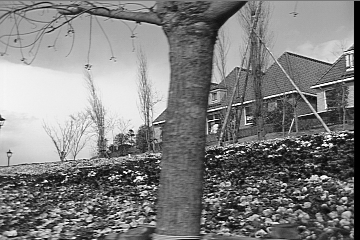
\includegraphics[width=0.82\textwidth]{imgs/FlowerGarden2.png}
  }{%
    \fbox{\parbox[c][5cm][c]{0.82\textwidth}{\centering Placeholder : \texttt{imgs/FlowerGarden2.png}}}
  }
  \caption{Fig Q1.1 -- Image originale.}
  \label{fig:q1-original}
\end{figure}

\begin{figure}[H]
  \centering
  \IfFileExists{imgs/metodo_directo.png}{%
    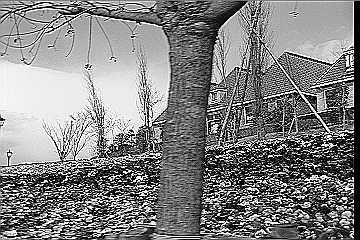
\includegraphics[width=0.82\textwidth]{imgs/metodo_directo.png}
  }{%
    \fbox{\parbox[c][5cm][c]{0.82\textwidth}{\centering Placeholder : \texttt{imgs/metodo_directo.png}}}
  }
  \caption{Fig Q1.2 -- Résultat méthode directe (\texttt{img2}).}
  \label{fig:q1-direct}
\end{figure}

\begin{figure}[H]
  \centering
  \IfFileExists{imgs/metodo_filter2d.png}{%
    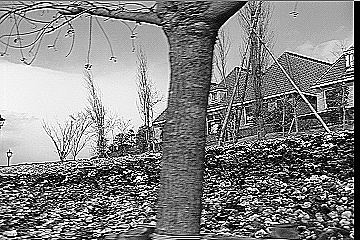
\includegraphics[width=0.82\textwidth]{imgs/metodo_filter2d.png}
  }{%
    \fbox{\parbox[c][5cm][c]{0.82\textwidth}{\centering Placeholder : \texttt{imgs/metodo_filter2d.png}}}
  }
  \caption{Fig Q1.3 -- Résultat \texttt{filter2D} après clipping (\texttt{img3\_clip}).}
  \label{fig:q1-filter2d-clip}
\end{figure}

% =========================================================
% Q2 — Rehaussement de contraste (interprétation fréquentielle)
% =========================================================
\subsection{Q2 --- Pourquoi le noyau r\'ealise un r\'ehaussement de contraste ?}
\label{sec:q2_rehaussement}

\subsubsection{Objectif}
Expliquer pourquoi le noyau de convolution utilis\'e en Q1 r\'ealise un r\'ehaussement de contraste, en reliant l'interpr\'etation spatiale (\(I-\Delta I\)) et l'interpr\'etation fr\'equentielle (renforcement des hautes fr\'equences).

\subsubsection{Rappels théoriques}
Le noyau utilis\'e dans l'exemple est :
\[
K=
\begin{bmatrix}
0 & -1 & 0\\
-1 & 5 & -1\\
0 & -1 & 0
\end{bmatrix}
\]
et le filtrage s'\'ecrit localement :
\[
I_f(x,y)=5I(x,y)-I(x\!-\!1,y)-I(x\!+\!1,y)-I(x,y\!-\!1)-I(x,y\!+\!1).
\]

Tout d'abord, la somme des coefficients vaut \(5-4=1\), ce qui implique un gain DC \'egal \`a 1 : sur une zone uniforme (tous les pixels \'egaux \`a une constante \(c\)), on obtient \(I_f=c\). Le filtre pr\'eserve donc globalement la luminance des r\'egions plates.

\subsubsection{Méthode / Implémentation}
Ensuite, ce noyau correspond \`a une accentuation par soustraction du Laplacien. Pour le Laplacien discret \`a 4-voisins :
\[
\Delta I = I(x\!-\!1,y)+I(x\!+\!1,y)+I(x,y\!-\!1)+I(x,y\!+\!1)-4I(x,y),
\]
on a :
\[
I-\Delta I = 5I(x,y)-\big(I(x\!-\!1,y)+I(x\!+\!1,y)+I(x,y\!-\!1)+I(x,y\!+\!1)\big),
\]
ce qui est exactement l'expression du filtre. Or, le Laplacien met en \'evidence les variations rapides d'intensit\'e (bords, d\'etails) : la combinaison \(I-\Delta I\) ajoute une composante passe-haut \`a l'image. Ainsi, les diff\'erences locales sont amplifi\'ees (un pixel plus clair que ses voisins devient encore plus clair, et inversement), ce qui produit un r\'ehaussement de contraste au voisinage des contours. Ce ph\'enom\`ene peut engendrer des valeurs hors de \([0,255]\) (overshoot/undershoot), justifiant l'usage d'une saturation (clipping) pour une visualisation en 8 bits.

Du point de vue fr\'equentiel, un filtrage spatial lin\'eaire correspond \`a une multiplication dans le domaine de Fourier :
\[
\widehat{I_f}(u,v)=\widehat{I}(u,v)\,\widehat{K}(u,v).
\]
Les basses fr\'equences (petits \(u,v\)) repr\'esentent les variations lentes (\'eclairage, r\'egions uniformes), tandis que les hautes fr\'equences correspondent aux variations rapides (bords, textures fines). Le Laplacien \'etant un op\'erateur de d\'erivation seconde, sa transform\'ee de Fourier est proportionnelle \`a \((u^2+v^2)\widehat{I}(u,v)\) (\'a un signe et une constante pr\`es), ce qui signifie qu'il amplifie les hautes fr\'equences et annule la composante continue. En cons\'equence, le filtre \(I-\Delta I\) garde un gain proche de 1 \`a tr\`es basse fr\'equence (coh\'erent avec \(\sum K = 1\)), mais augmente le gain lorsque \(\sqrt{u^2+v^2}\) cro\^it : les composantes hautes fr\'equences sont renforc\'ees, ce qui explique le r\'ehaussement de contraste observ\'e sur les contours.

\subsubsection{Résultats}
\textbf{Analyse qualitative.}
Le comportement attendu est un rehaussement du contraste local au voisinage des contours et textures fines, avec pr\'eservation globale des zones uniformes (gain DC unit\'e). Cette accentuation peut produire des valeurs hors de \([0,255]\) (overshoot/undershoot), ce qui motive l'usage d'un clipping pour un affichage 8 bits.

\subsubsection{Discussion}
L'interpr\'etation spatiale (\(I-\Delta I\)) et l'interpr\'etation fr\'equentielle (\(\widehat{I_f}=\widehat{I}\,\widehat{K}\)) sont coh\'erentes : le filtre conserve les basses fr\'equences utiles \`a la luminance globale et renforce les hautes fr\'equences responsables des bords, d'o\`u l'effet de nettete per\c cu.

\subsubsection{Figures}
\begin{formal}
\textbf{TODO -- Figures Q2}
\begin{itemize}[leftmargin=1.5em]
  \item TODO: ajouter figure du r\'esultat \textit{sharpened} (si disponible).
  \item TODO: ajouter histogramme avant/apr\`es (si disponible).
\end{itemize}
\end{formal}

% =========================================================
% Q3 — Gradients (Ix, Iy) et norme ||∇I||
% =========================================================
\subsection{Q3 --- Approximation du gradient par convolution et pr\'ecautions d'affichage}
\label{sec:q3_gradients}

\subsubsection{Objectif}
L'objectif est d'approximer les composantes du gradient d'une image en niveaux de gris
\[
I_x(x,y) \approx \frac{\partial I}{\partial x}(x,y), 
\qquad
I_y(x,y) \approx \frac{\partial I}{\partial y}(x,y),
\]
puis de calculer la norme euclidienne
\[
\|\nabla I(x,y)\| = \sqrt{I_x(x,y)^2 + I_y(x,y)^2}.
\]

\subsubsection{Rappels théoriques}
Nous utilisons les noyaux de Sobel \(3\times3\), qui combinent une d\'erivation et un l\'eger lissage (plus robuste au bruit qu'une simple diff\'erence finie) :
\[
K_x=
\begin{bmatrix}
-1 & 0 & 1\\
-2 & 0 & 2\\
-1 & 0 & 1
\end{bmatrix},
\qquad
K_y=
\begin{bmatrix}
-1 & -2 & -1\\
0 & 0 & 0\\
1 & 2 & 1
\end{bmatrix}.
\]

\subsubsection{Méthode / Implémentation}
Les convolutions sont r\'ealis\'ees avec \texttt{cv2.filter2D} (profondeur \texttt{CV\_64F}) et une gestion de bord \texttt{BORDER\_REPLICATE}.

\subsubsection{Résultats}
Sur l'image test (\(240\times 360\)), nous obtenons :
\[
I_x \in [-879,\;730],\qquad
I_y \in [-1012,\;974],\qquad
\|\nabla I\| \in [0,\;1070.29].
\]
Le signe de \(I_x\) et \(I_y\) d\'epend de la direction du changement d'intensit\'e (clair$\rightarrow$fonc\'e vs fonc\'e$\rightarrow$clair). Dans la zone int\'erieure (hors bord), la r\'epartition est quasi \'equilibr\'ee :
\[
I_x:\; 50.76\% \text{ n\'egatifs},\; 46.52\% \text{ positifs},\; 2.71\% \text{ z\'eros},
\]
\[
I_y:\; 45.84\% \text{ n\'egatifs},\; 51.85\% \text{ positifs},\; 2.31\% \text{ z\'eros}.
\]
Ces statistiques confirment que les composantes du gradient sont \`a valeurs sign\'ees (donc incompatibles avec un affichage direct en 8 bits non sign\'e).
\[
M_x = 455,\qquad M_y = 682.97,\qquad M_g = P_{99}(\|\nabla I\|)=722.12.
\]

\subsubsection{Discussion}
\textbf{Interpr\'etation qualitative.}
La carte \(I_x\) met en \'evidence les variations horizontales (donc les \emph{bords verticaux}), tandis que \(I_y\) r\'epond aux variations verticales (donc les \emph{bords horizontaux}).
La norme \(\|\nabla I\|\) fournit une mesure scalaire de \og force de bord \fg{}, ind\'ependante de l'orientation, et donc plus facile \`a interpr\'eter pour la d\'etection de contours.

\textbf{Pr\'ecautions pour un affichage correct (valeurs n\'egatives et positives).}
Pour visualiser correctement \(I_x\) et \(I_y\) \emph{dans tous les cas} :
\begin{itemize}
  \item \textbf{Conserver un type flottant} (\texttt{float64} ici). Un passage pr\'ematur\'e en \texttt{uint8} provoquerait une saturation ou un \emph{wrap-around} des valeurs n\'egatives.
  \item \textbf{Ne pas clipper} \(I_x\) et \(I_y\) dans \([0,255]\) avant affichage, sous peine de perdre l'information de signe.
  \item \textbf{Utiliser une colormap divergente} centr\'ee en \(0\) et une \textbf{\'echelle sym\'etrique} : \(v_{\min}=-M\), \(v_{\max}=+M\), afin que le z\'ero corresponde \`a une couleur neutre et que les amplitudes positives/n\'egatives soient comparables.
  \item \textbf{Choisir \(M\) de mani\`ere robuste} (percentile) pour \'eviter qu'un petit nombre de valeurs extr\^emes \og \'ecrase \fg{} la dynamique. Ici, nous utilisons \(p=99\%\) sur la zone int\'erieure :
  \[
  M_x = 455,\qquad M_y = 682.97.
  \]
  \item Pour \(\|\nabla I\|\) (toujours \(\ge 0\)), utiliser une colormap en niveaux de gris avec \(v_{\min}=0\) et un \textbf{maximum robuste} :
  \[
  M_g = P_{99}(\|\nabla I\|)=722.12,
  \]
  afin de conserver une image lisible.
\end{itemize}

\subsubsection{Figures}
Les figures suivantes illustrent (i) les composantes sign\'ees \(I_x\) et \(I_y\) (colormap divergente) et (ii) leurs amplitudes \(|I_x|\), \(|I_y|\) ainsi que la norme \(\|\nabla I\|\), qui met en \'evidence les contours ind\'ependamment de l'orientation.

\begin{figure}[H]
  \centering
  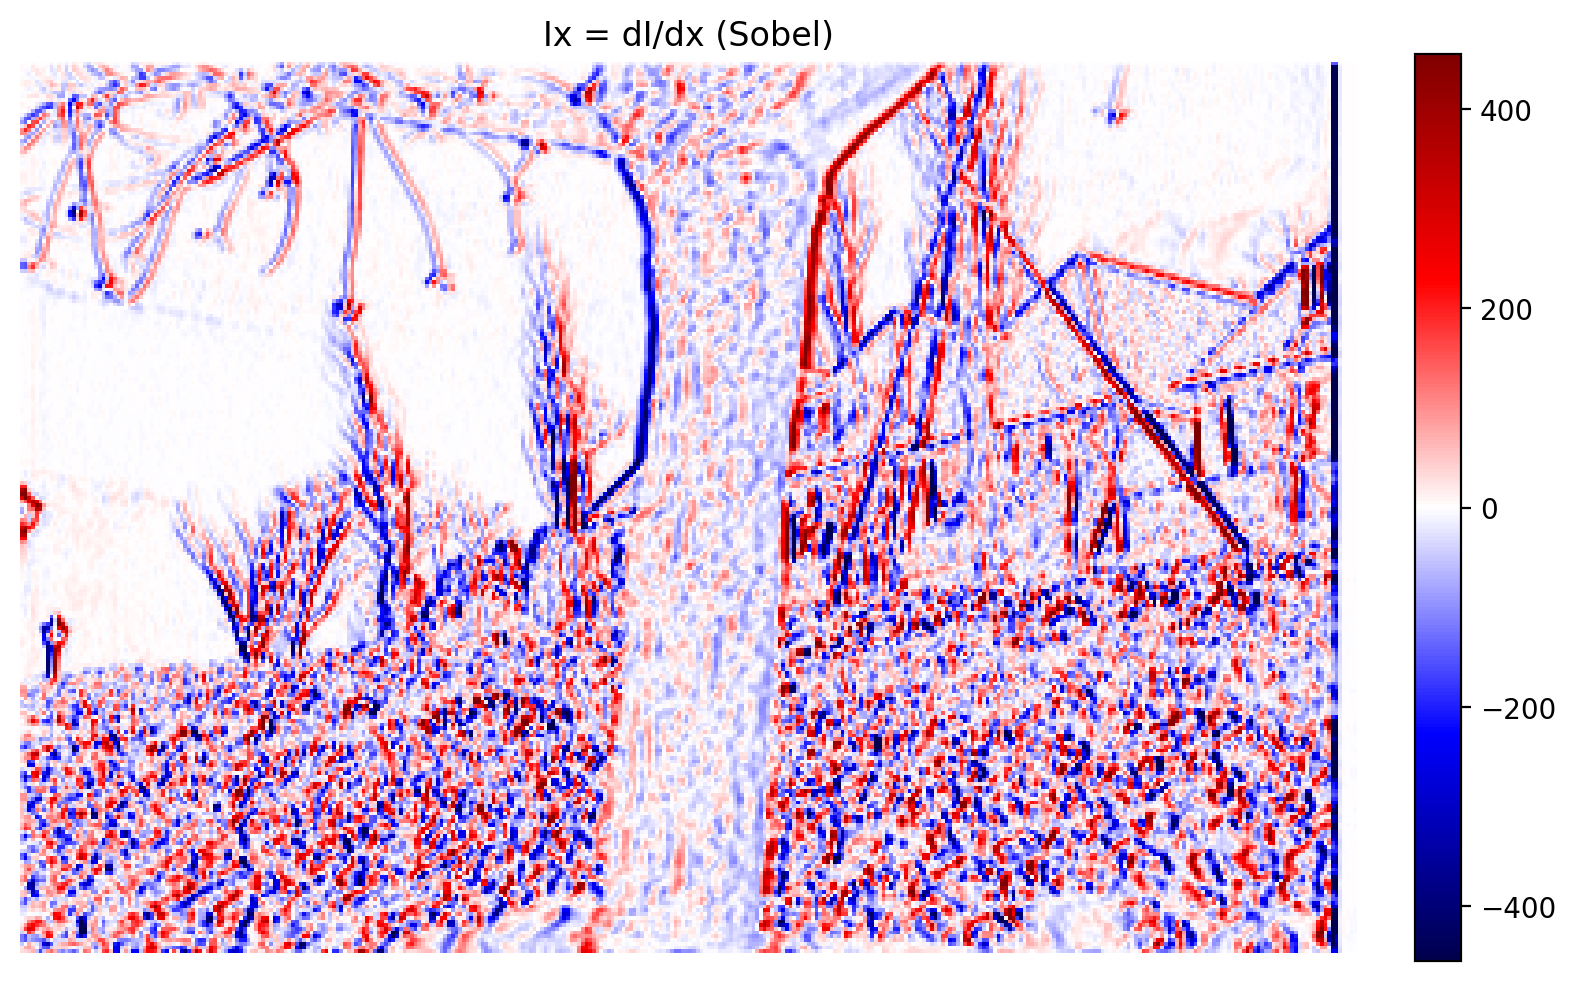
\includegraphics[width=0.95\linewidth]{imgs/Q3/q3_Ix.png}
  \caption{\(I_x = \partial I/\partial x\) (Sobel). La colormap divergente centr\'ee en 0 met en \'evidence les variations horizontales (bords verticaux).}
  \label{fig:q3_ix}
\end{figure}

\begin{figure}[H]
  \centering
  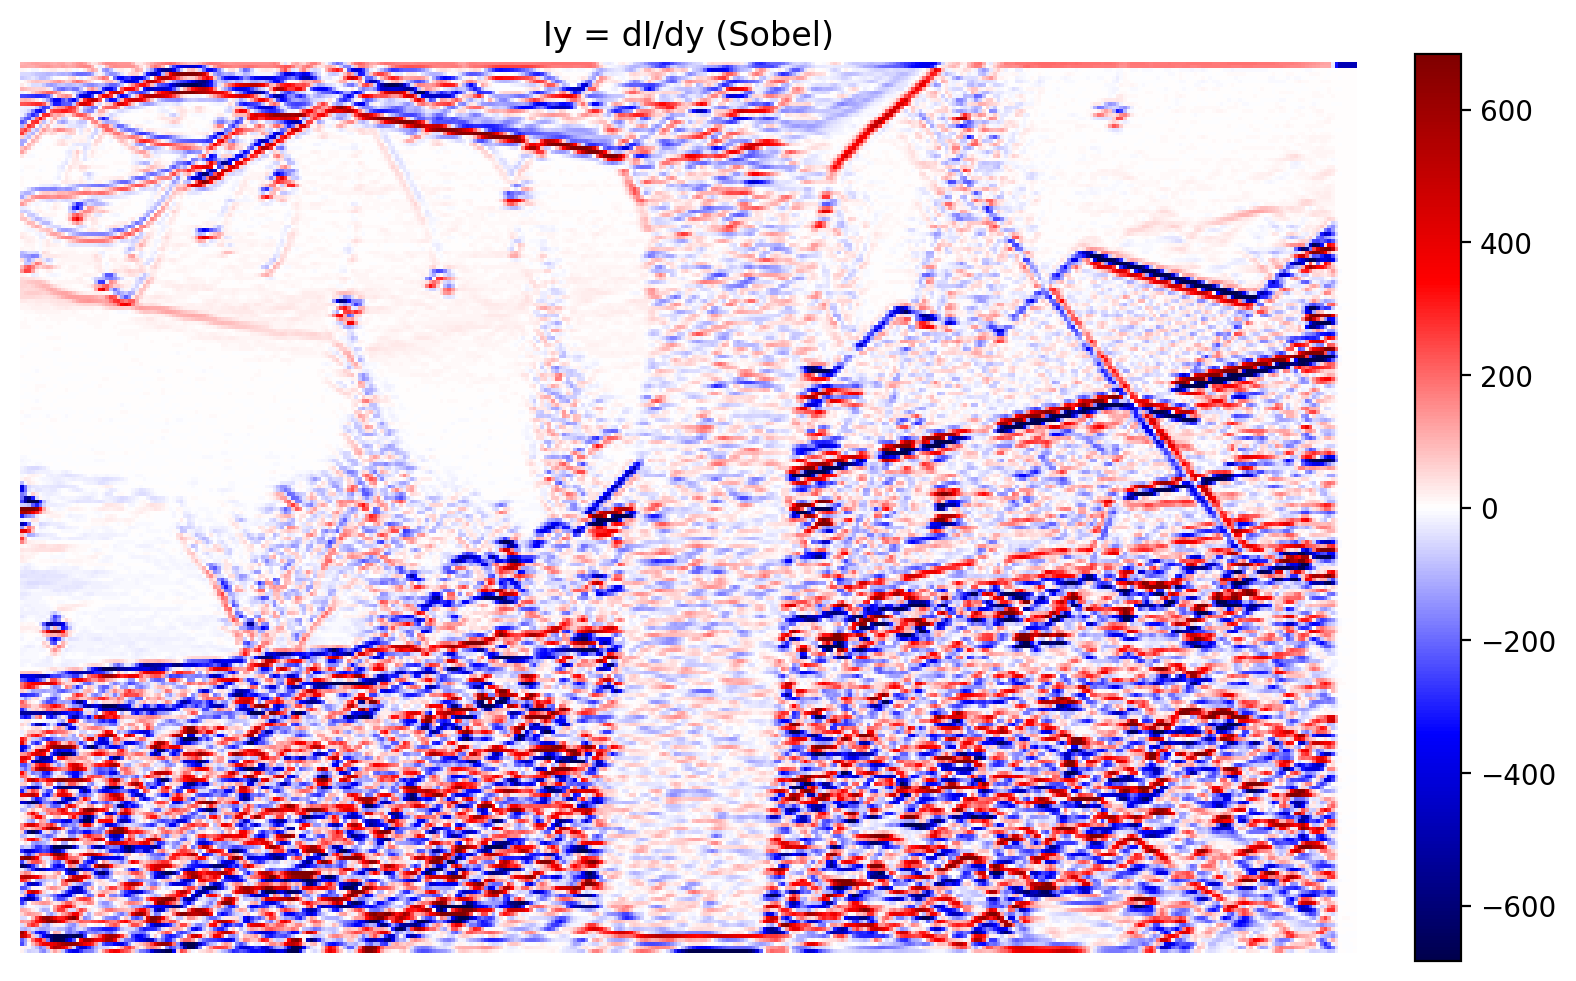
\includegraphics[width=0.95\linewidth]{imgs/Q3/q3_Iy.png}
  \caption{\(I_y = \partial I/\partial y\) (Sobel). La colormap divergente centr\'ee en 0 met en \'evidence les variations verticales (bords horizontaux).}
  \label{fig:q3_iy}
\end{figure}

\begin{figure}[H]
  \centering
  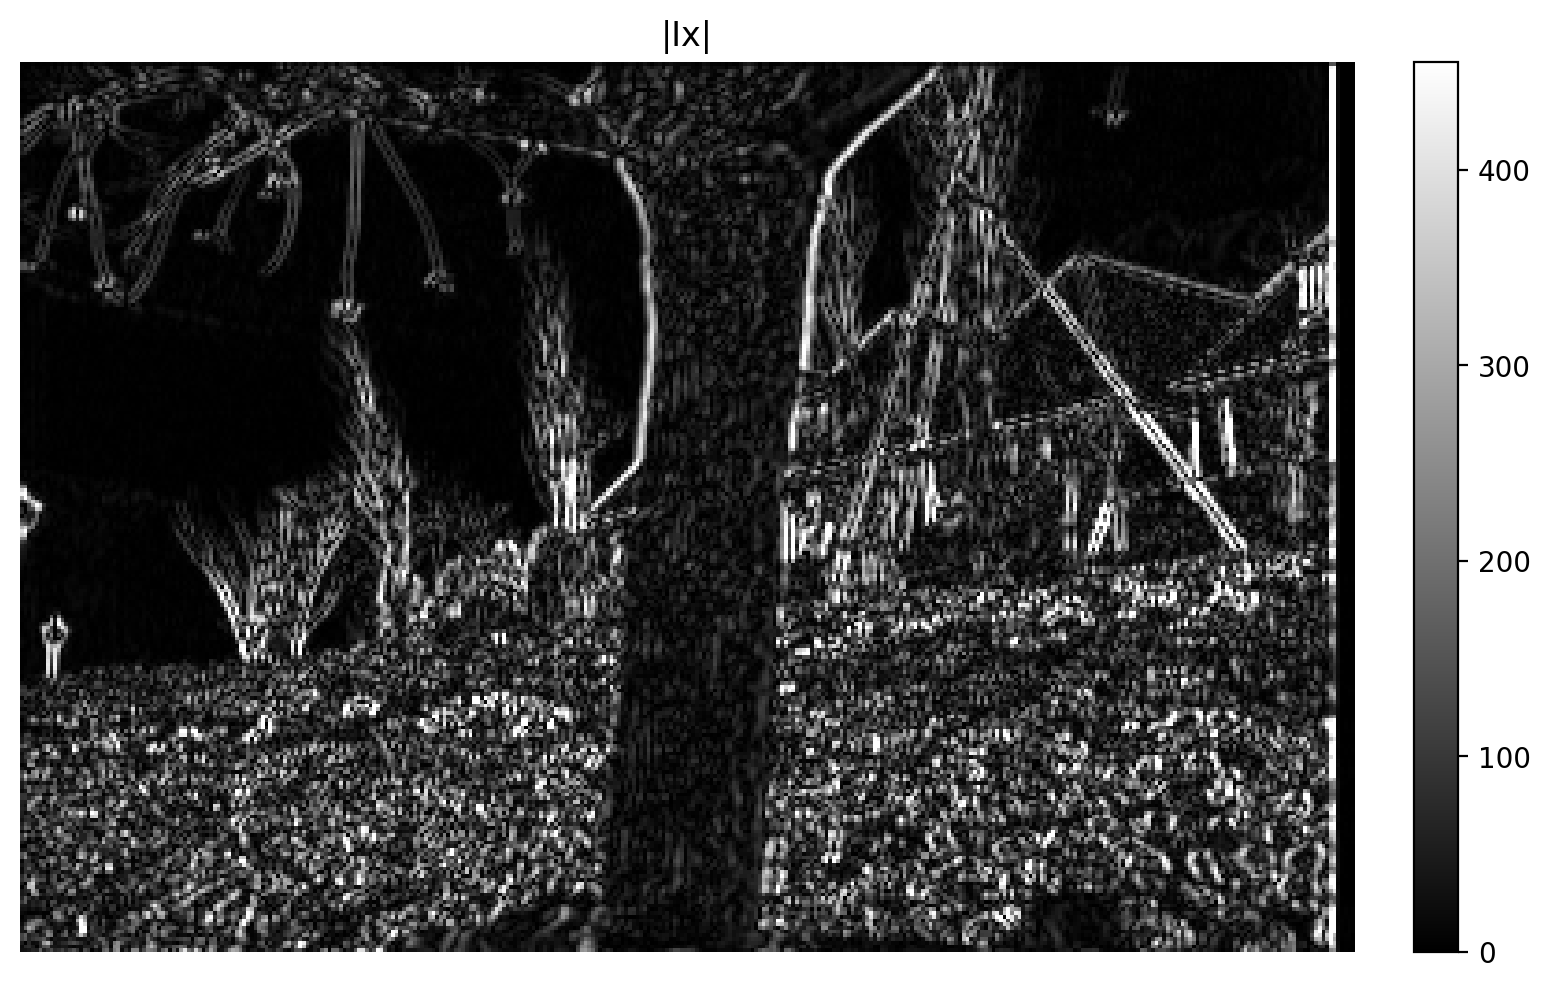
\includegraphics[width=0.95\linewidth]{imgs/Q3/q3_abs_Ix.png}
  \caption{Amplitude \(|I_x|\). En supprimant le signe, on visualise directement l'intensit\'e des variations horizontales.}
  \label{fig:q3_abs_ix}
\end{figure}

\begin{figure}[H]
  \centering
  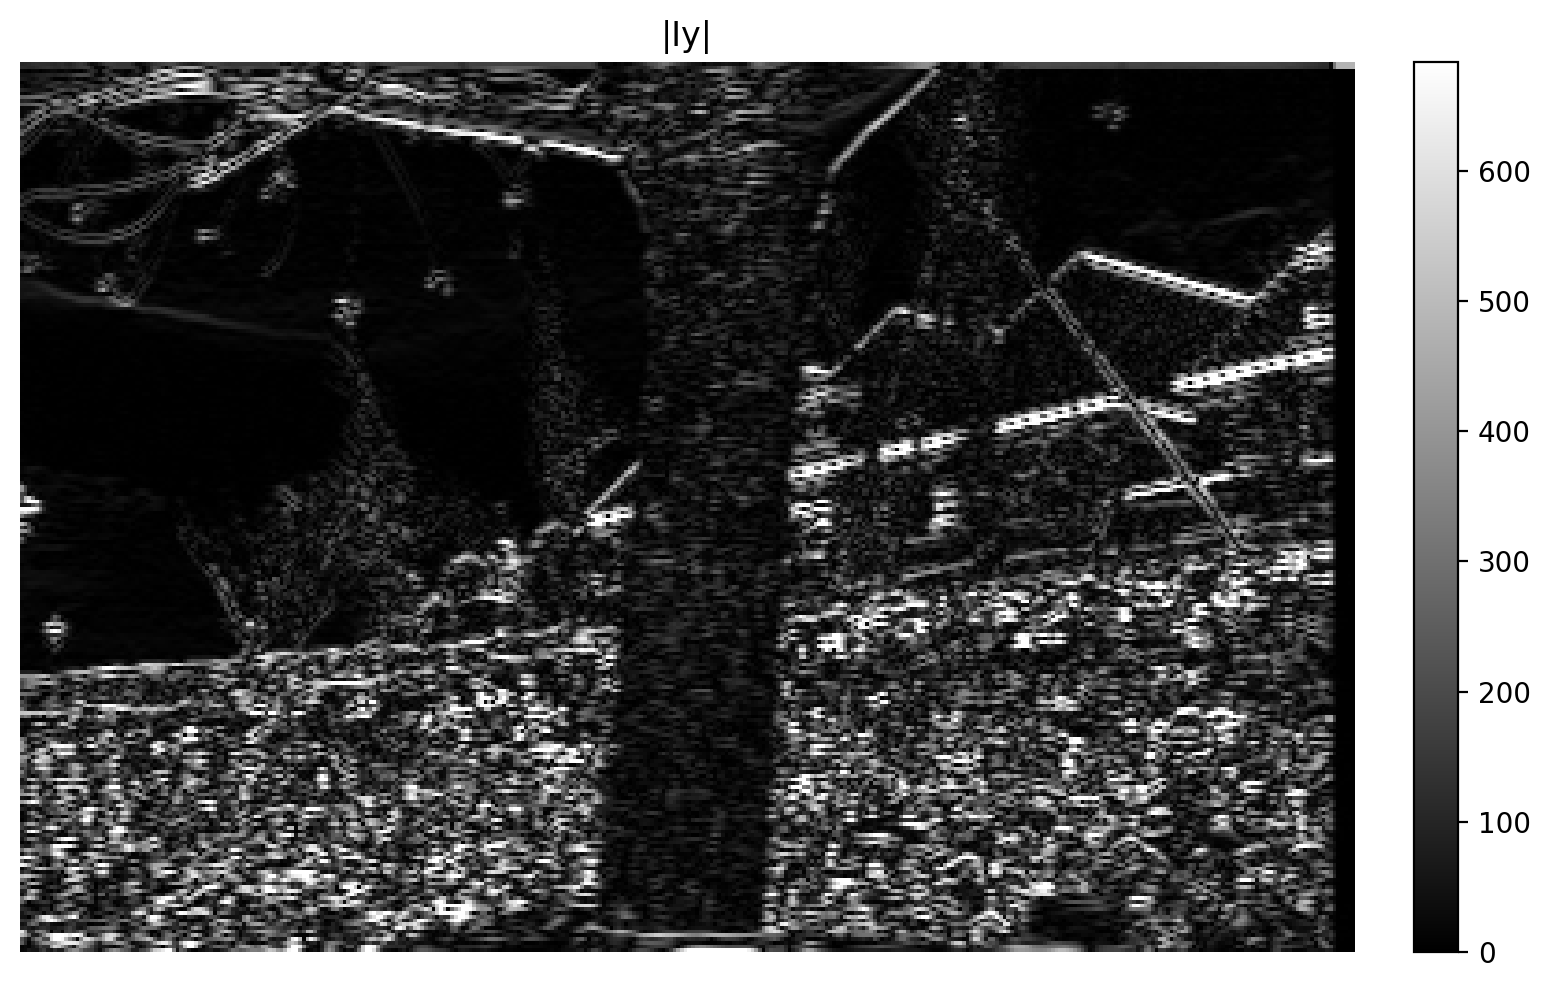
\includegraphics[width=0.95\linewidth]{imgs/Q3/q3_abs_Iy.png}
  \caption{Amplitude \(|I_y|\). Les zones textur\'ees et les bords horizontaux pr\'esentent une r\'eponse plus forte.}
  \label{fig:q3_abs_iy}
\end{figure}

\begin{figure}[H]
  \centering
  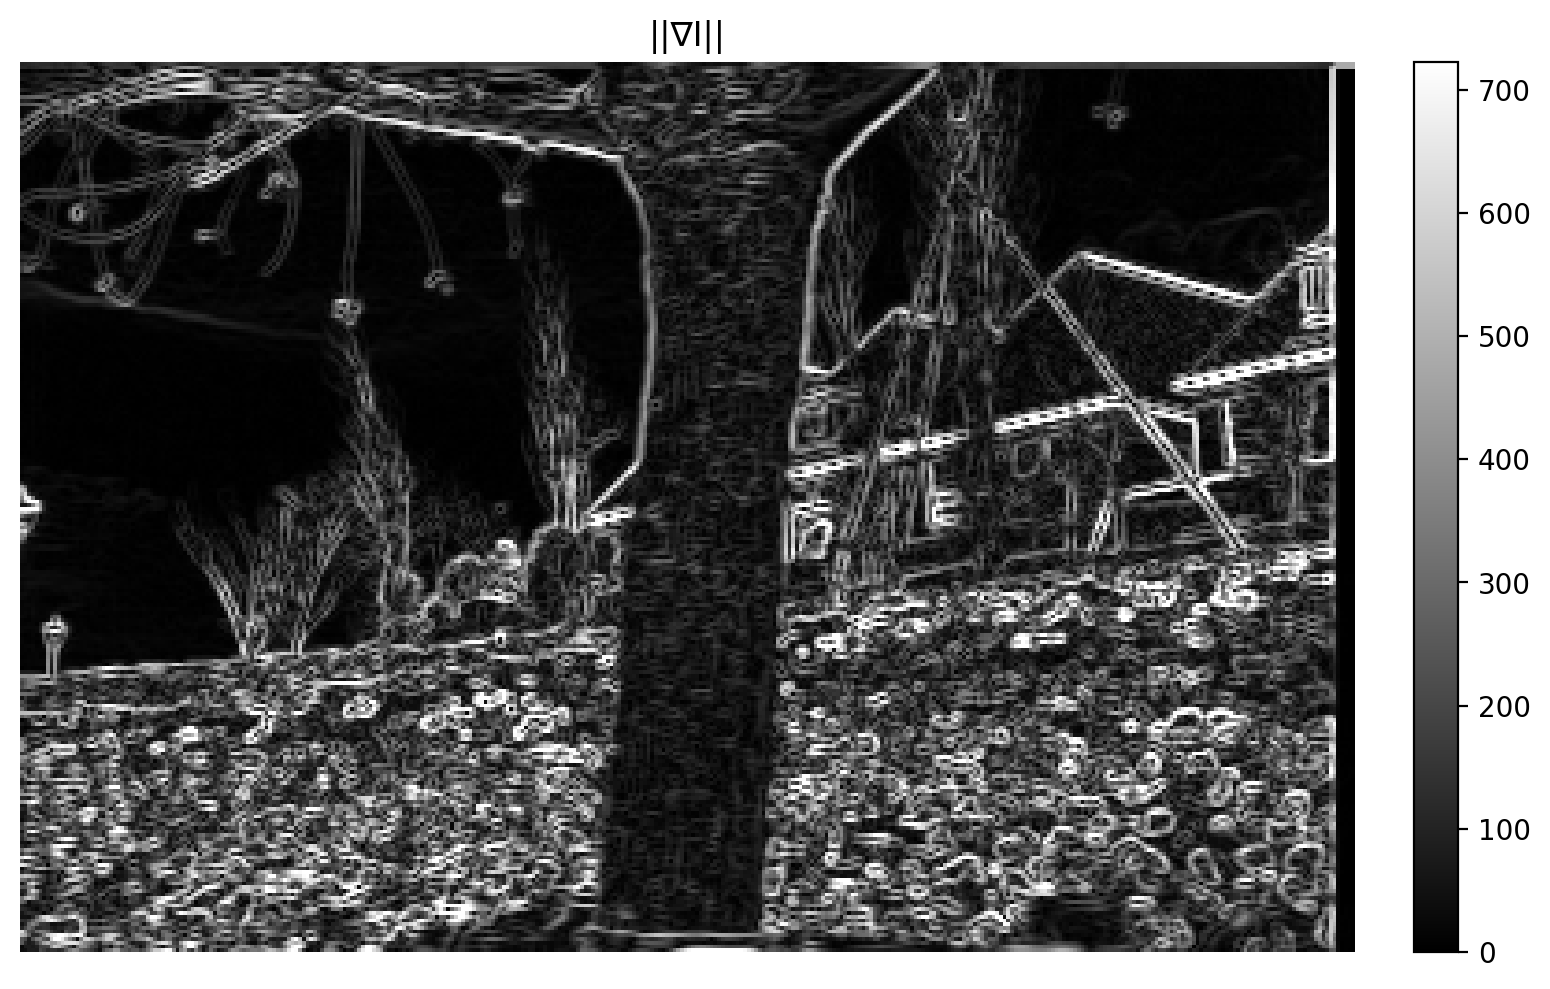
\includegraphics[width=0.95\linewidth]{imgs/Q3/q3_grad_norm.png}
  \caption{Norme du gradient \(\|\nabla I\|\). Cette carte scalaire (toujours positive) r\'esume la force des contours ind\'ependamment de leur orientation.}
  \label{fig:q3_grad_norm}
\end{figure}

% ====================================================
% PARTIE 3
% ====================================================
\section{(3) Détecteurs : Q4--Q6}

\subsection{Q4 --- Détecteur de Harris : compléments d'implémentation}

\subsubsection{Rappels théoriques}
Le détecteur de Harris repose sur l'analyse des variations locales d'intensité selon les deux directions de l'image. À partir de l'image en niveaux de gris \(I(x,y)\), on calcule les dérivées spatiales \(I_x\) et \(I_y\). Ces dérivées alimentent ensuite la matrice d'autocorrélation locale, ou matrice des moments d'ordre deux,
\[
\Xi(x,y)=
\begin{bmatrix}
\sum_W I_x^2 & \sum_W I_x I_y \\
\sum_W I_x I_y & \sum_W I_y^2
\end{bmatrix},
\]
où la somme est effectuée sur une fenêtre locale \(W\) centrée au point \((x,y)\). Cette matrice résume la manière dont l'intensité varie dans le voisinage considéré. Une forte variation dans une seule direction caractérise plutôt un bord, tandis qu'une forte variation dans deux directions distinctes correspond à un coin, donc à un point d'intérêt.

La fonction d'intérêt de Harris s'écrit alors
\[
\Theta(x,y)=\det(\Xi)-\alpha\,\mathrm{trace}(\Xi)^2,
\]
avec \(\alpha > 0\). Lorsque \(\det(\Xi)\) est élevée et que les deux valeurs propres de \(\Xi\) sont simultanément importantes, \(\Theta\) prend de fortes valeurs positives, ce qui signale une structure localement saillante de type coin.

\subsubsection{Implémentation réalisée}
L'implémentation a été réalisée sur l'image \texttt{Graffiti0.png}, de taille \(320 \times 400\), lue en niveaux de gris puis convertie en \texttt{float64} afin de conserver une dynamique numérique compatible avec les calculs de dérivées et de produits. Le traitement est effectué à une seule échelle, avec une fenêtre locale fixe.

Les gradients \(I_x\) et \(I_y\) sont calculés par l'opérateur de Sobel de taille \(3 \times 3\), respectivement selon \(x\) et selon \(y\). À partir de ces dérivées, le script construit les trois termes élémentaires \(I_x^2\), \(I_y^2\) et \(I_x I_y\). La sommation locale sur la fenêtre \(W\) est ensuite réalisée par \texttt{cv2.boxFilter} avec \(\texttt{ksize}=(5,5)\) et \texttt{normalize=False}, ce qui fournit directement les quantités
\[
S_{xx}=\sum_W I_x^2,\qquad
S_{yy}=\sum_W I_y^2,\qquad
S_{xy}=\sum_W I_x I_y.
\]
Le tenseur de structure local est donc évalué sur une fenêtre carrée fixe de taille \(5 \times 5\). Le paramètre de Harris utilisé dans le code est \(\alpha = 0.04\), et la réponse finale est calculée sous la forme
\[
\det = S_{xx}S_{yy}-S_{xy}^2,\qquad
\mathrm{trace}=S_{xx}+S_{yy},\qquad
\Theta=\det-\alpha\,\mathrm{trace}^2.
\]
Cette écriture relie directement la formulation théorique au calcul numérique effectué dans \texttt{Harris.py}.

\subsubsection{Maxima locaux par dilatation morphologique}
Après calcul de \(\Theta\), le script extrait les points d'intérêt en recherchant des maxima locaux dans un voisinage \(3 \times 3\), défini par un élément structurant plein. La dilatation morphologique
\[
\Theta_{\mathrm{dil}} = \mathrm{dilate}(\Theta, se)
\]
remplace chaque pixel par la valeur maximale de \(\Theta\) dans ce voisinage. Par construction, si un pixel est strictement inférieur à la valeur dilatée au même emplacement, cela signifie qu'il existe dans son voisinage au moins un autre pixel portant une réponse plus forte. Il ne peut donc pas correspondre à un maximum local.

La ligne
\begin{formal}
\texttt{Theta\_maxloc[Theta < Theta\_dil] = 0.0}
\end{formal}
supprime précisément tous ces pixels non maximaux. Inversement, les pixels qui conservent une valeur égale au maximum de leur voisinage ne sont pas annulés et constituent les candidats maxima locaux. Cette étape revient donc à comparer \(\Theta\) à son enveloppe locale maximale produite par la dilatation.

Un second filtrage est ensuite appliqué par seuil relatif :
\begin{formal}
\texttt{Theta\_maxloc[Theta < seuil\_relatif * Theta.max()] = 0.0}
\end{formal}
avec \(\texttt{seuil\_relatif}=0.01\). Cette opération élimine les réponses trop faibles, même si elles sont localement maximales, ce qui évite de conserver des pics peu significatifs dus au bruit ou à de faibles variations de texture. La combinaison suppression des non-maxima et seuillage produit ainsi une sélection de points plus stable et spatialement plus pertinente.

\subsubsection{Résultats et interprétation}
L'exécution sur \texttt{Graffiti0.png} fournit un temps de calcul de \SI{0.012387734}{s}, soit \num{96.779171875} cycles par pixel, ce qui reste rapide pour une image de taille modérée (\(320 \times 400\)) et une implémentation reposant uniquement sur des opérateurs OpenCV standards. Le nombre de points de Harris détectés après seuillage est de \(624\), ce qui constitue un ensemble suffisamment dense pour décrire les structures saillantes de l'image sans produire une couverture uniformément diffuse.

L'analyse visuelle de la carte \(\Theta\) montre des pics localisés plutôt qu'une activation homogène, ce qui est conforme au comportement attendu du critère de Harris. Les zones relativement homogènes restent peu activées, tandis que les réponses fortes se concentrent sur des coins, des intersections et des changements de direction marqués. Sur l'image de graffiti, de nombreux points sont détectés sur les contours structurés du personnage ainsi que sur plusieurs détails texturés du décor. Le nombre de pixels marqués pour l'affichage (\(5237\)) est logiquement plus élevé que le nombre de points détectés, car la dilatation finale avec un élément en forme de croix sert uniquement à rendre les points visibles sur l'image couleur.

\subsubsection{Figure}
\begin{figure}[H]
  \centering
  \IfFileExists{imgs/Q4/q4_harris_image_originale.png}{%
    \begin{minipage}[t]{0.32\textwidth}
      \centering
      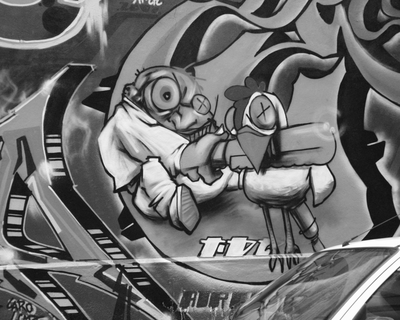
\includegraphics[width=\linewidth]{imgs/Q4/q4_harris_image_originale.png}
      \vspace{0.3em}

      \small Image originale
    \end{minipage}\hfill
    \begin{minipage}[t]{0.32\textwidth}
      \centering
      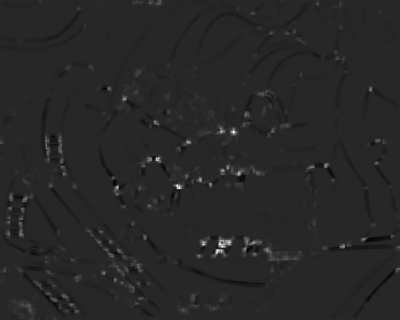
\includegraphics[width=\linewidth]{imgs/Q4/q4_harris_fonction_harris.png}
      \vspace{0.3em}

      \small Fonction de Harris
    \end{minipage}\hfill
    \begin{minipage}[t]{0.32\textwidth}
      \centering
      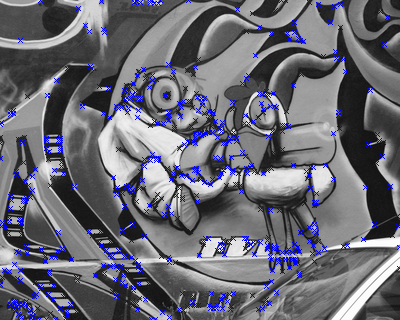
\includegraphics[width=\linewidth]{imgs/Q4/q4_harris_points_harris.png}
      \vspace{0.3em}

      \small Points de Harris
    \end{minipage}
  }{%
    \fbox{\parbox[c][4cm][c]{0.9\textwidth}{\centering Figures Q4 absentes : générer d'abord les images \texttt{q4\_harris\_*.png} dans \texttt{docs/imgs/Q4}.}}
  }
  \caption{Détection de Harris sur \texttt{Graffiti0.png}. De gauche à droite : image d'origine en niveaux de gris, carte de réponse \(\Theta\) normalisée pour la visualisation, puis superposition des points d'intérêt détectés après suppression des non-maxima locaux et seuillage relatif.}
  \label{fig:q4-harris}
\end{figure}

La figure~\ref{fig:q4-harris} confirme que l'implémentation reproduit le comportement attendu du détecteur de Harris à fenêtre fixe : la réponse est concentrée sur des structures réellement informatives, et la chaîne ``fenêtre locale + critère de Harris + suppression des non-maxima'' produit une détection spatialement cohérente sur l'image de graffiti, sans activation parasite généralisée dans les zones peu structurées.

\subsection{Q5 --- Harris : paramètres, multi-échelles et contrainte de distance}

\subsubsection{Objectif et protocole}
Cette partie étudie l'influence de la taille de la fenêtre de sommation \(W\) et du paramètre \(\alpha\) sur la réponse de Harris, avant de discuter deux prolongements classiques : le calcul multi-échelles et l'extension de la notion de maximum local sous contrainte de distance minimale. Les expériences ont été réalisées sur \texttt{Graffiti0.png} en conservant constants le voisinage de suppression des non-maxima (\(3 \times 3\)) et le seuil relatif (\(0.01\)), avec \(W \in \{3,5,7,9\}\) et \(\alpha \in \{0.04,0.05,0.06\}\).

\subsubsection{Analyse des résultats expérimentaux}
Le tableau~\ref{tab:q5-metrics} synthétise quelques configurations représentatives, tandis que les figures~\ref{fig:q5-window} et~\ref{fig:q5-alpha} permettent de croiser les mesures numériques avec l'observation des points détectés et des cartes \(\Theta\).

\begin{table}[H]
  \centering
  \caption{Q5 -- Configurations représentatives pour l'analyse des paramètres de Harris.}
  \label{tab:q5-metrics}
  \footnotesize
  \begin{tabular}{@{}rrrrrr@{}}
    \toprule
    \(W\) & \(\alpha\) & Points détectés & Pixels marqués & Temps (s) & CPP \\
    \midrule
    3 & 0.05 & 651 & 5453 & 0.005896867 & 46.0693 \\
    5 & 0.05 & 607 & 5097 & 0.003622706 & 28.3024 \\
    7 & 0.05 & 524 & 4392 & 0.003871695 & 30.2476 \\
    9 & 0.05 & 521 & 4335 & 0.005206661 & 40.6770 \\
    5 & 0.04 & 624 & 5237 & 0.003369293 & 26.3226 \\
    5 & 0.06 & 579 & 4874 & 0.003962638 & 30.9581 \\
    \bottomrule
  \end{tabular}
\end{table}

L'effet de \(W\) apparaît d'abord comme le plus structurant. À \(\alpha=0.05\) fixé, le nombre de points détectés passe de \(651\) pour \(W=3\) à \(521\) pour \(W=9\), soit une baisse d'environ \(20.0\%\). La même tendance se retrouve pour les autres valeurs de \(\alpha\) : selon le CSV, le passage de \(W=3\) à \(W=9\) fait perdre entre \(123\) et \(151\) points, soit \(19.5\%\) à \(22.3\%\) des détections initiales. Visuellement, la ligne supérieure de la figure~\ref{fig:q5-window} montre que l'augmentation de \(W\) élimine une partie des détections diffuses situées sur des parois faiblement texturées et le long de contours allongés qui relèvent davantage du bord que du coin. La carte \(\Theta\) se stabilise simultanément : sur la ligne inférieure, les réponses deviennent moins granuleuses et davantage concentrées en pics compacts. Cette meilleure robustesse s'accompagne toutefois d'un coût en localisation fine. Sur quelques coins serrés du motif central et du lettrage inférieur, la croix retenue se décale légèrement par rapport au coin visuel, et certaines structures encore détectées pour \(W=3\) ou \(W=5\) disparaissent lorsque \(W\) devient trop grand. Autrement dit, une fenêtre large améliore la sélectivité et réduit les fausses alarmes sur les bords, mais elle lisse aussi des structures fines et peut faire perdre des coins pertinents.

La variation de \(\alpha\) agit de manière plus progressive. À \(W=5\) fixé, le nombre de points détectés passe de \(624\) pour \(\alpha=0.04\) à \(579\) pour \(\alpha=0.06\), soit une réduction de \(7.2\%\), très inférieure à celle provoquée par la variation de \(W\). Sur l'ensemble du CSV, l'écart entre \(\alpha=0.04\) et \(\alpha=0.06\) reste compris entre \(19\) et \(47\) points selon \(W\), soit \(3.6\%\) à \(7.2\%\). La figure~\ref{fig:q5-alpha} confirme que l'augmentation de \(\alpha\) nettoie certaines réponses faibles sur les surfaces peu texturées et supprime plusieurs fausses détections alignées avec des bords, mais sans modifier aussi brutalement la répartition spatiale globale. Les coins majeurs du visage, des contours circulaires et de la zone inférieure restent pour la plupart présents, et la position des croix demeure globalement stable d'une valeur de \(\alpha\) à l'autre. Les cartes \(\Theta\) montrent le même phénomène : l'augmentation de \(\alpha\) atténue des activations diffuses, tout en conservant les maxima principaux. En pratique, \(\alpha\) joue donc le rôle d'un paramètre de sélection plus fin, moins brutal que \(W\).

Les mesures de temps corroborent ce caractère secondaire du réglage des paramètres vis-à-vis de la densité de points. Hormis une exécution à \(W=3\), \(\alpha=0.04\) mesurée à \SI{0.017730799}{s}, nettement au-dessus du reste du tableau, tous les autres temps se situent entre \SI{0.003232796}{s} et \SI{0.005206661}{s}. Ce point isolé doit être interprété avec prudence : les autres expériences ne montrent pas d'augmentation monotone du temps de calcul qui permettrait d'en faire une tendance robuste. En revanche, le nombre de pixels marqués suit bien l'évolution du nombre de points détectés, ce qui confirme que la raréfaction des points observée sur les figures ne relève pas seulement d'un effet d'affichage.

\begin{figure}[H]
  \centering
  \IfFileExists{imgs/Q5/q5_harris_points_q5_ws3_a0p05_m3_t0p01.png}{%
    \begin{minipage}[t]{0.24\textwidth}
      \centering
      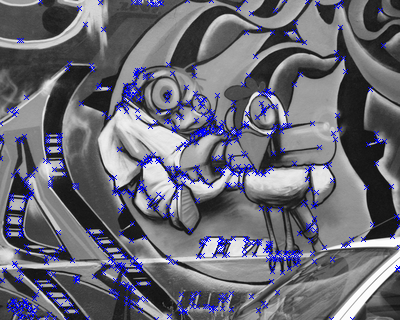
\includegraphics[width=\linewidth]{imgs/Q5/q5_harris_points_q5_ws3_a0p05_m3_t0p01.png}
      \vspace{0.3em}

      \small Points, \(W=3\)
    \end{minipage}\hfill
    \begin{minipage}[t]{0.24\textwidth}
      \centering
      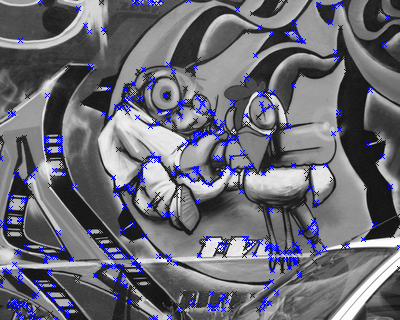
\includegraphics[width=\linewidth]{imgs/Q5/q5_harris_points_q5_ws5_a0p05_m3_t0p01.png}
      \vspace{0.3em}

      \small Points, \(W=5\)
    \end{minipage}\hfill
    \begin{minipage}[t]{0.24\textwidth}
      \centering
      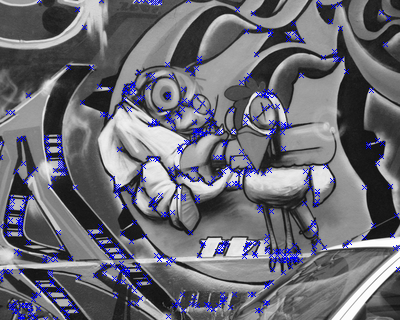
\includegraphics[width=\linewidth]{imgs/Q5/q5_harris_points_q5_ws7_a0p05_m3_t0p01.png}
      \vspace{0.3em}

      \small Points, \(W=7\)
    \end{minipage}\hfill
    \begin{minipage}[t]{0.24\textwidth}
      \centering
      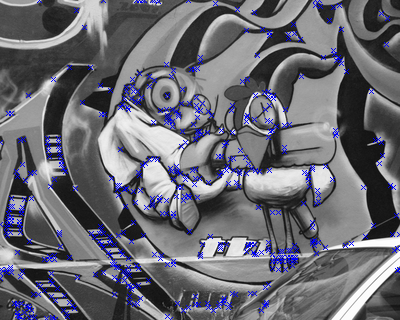
\includegraphics[width=\linewidth]{imgs/Q5/q5_harris_points_q5_ws9_a0p05_m3_t0p01.png}
      \vspace{0.3em}

      \small Points, \(W=9\)
    \end{minipage}

    \vspace{0.8em}

    \begin{minipage}[t]{0.24\textwidth}
      \centering
      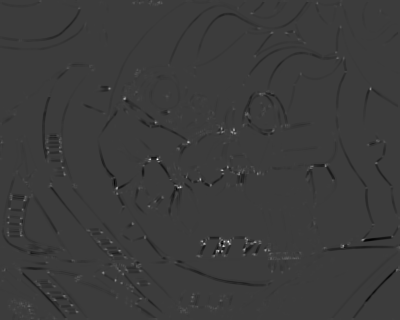
\includegraphics[width=\linewidth]{imgs/Q5/q5_harris_theta_q5_ws3_a0p05_m3_t0p01.png}
      \vspace{0.3em}

      \small \(\Theta\), \(W=3\)
    \end{minipage}\hfill
    \begin{minipage}[t]{0.24\textwidth}
      \centering
      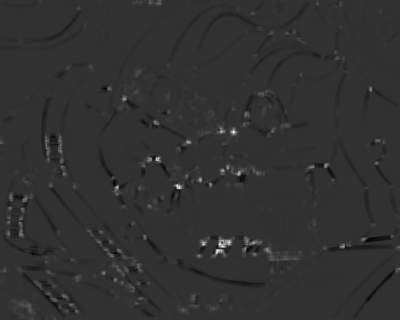
\includegraphics[width=\linewidth]{imgs/Q5/q5_harris_theta_q5_ws5_a0p05_m3_t0p01.png}
      \vspace{0.3em}

      \small \(\Theta\), \(W=5\)
    \end{minipage}\hfill
    \begin{minipage}[t]{0.24\textwidth}
      \centering
      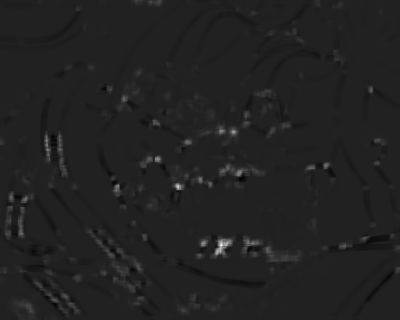
\includegraphics[width=\linewidth]{imgs/Q5/q5_harris_theta_q5_ws7_a0p05_m3_t0p01.png}
      \vspace{0.3em}

      \small \(\Theta\), \(W=7\)
    \end{minipage}\hfill
    \begin{minipage}[t]{0.24\textwidth}
      \centering
      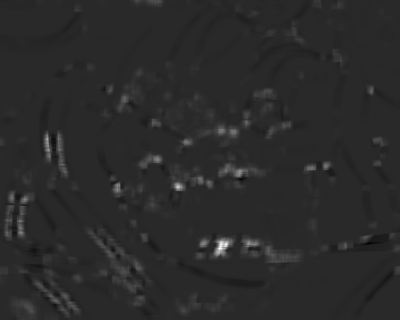
\includegraphics[width=\linewidth]{imgs/Q5/q5_harris_theta_q5_ws9_a0p05_m3_t0p01.png}
      \vspace{0.3em}

      \small \(\Theta\), \(W=9\)
    \end{minipage}
  }{%
    \fbox{\parbox[c][7cm][c]{0.95\textwidth}{\centering Figures Q5 absentes : générer d'abord les images \texttt{q5\_harris\_points\_*} et \texttt{q5\_harris\_theta\_*} dans \texttt{docs/imgs/Q5}.}}
  }
  \caption{Influence de la taille de fenêtre de sommation \(W\) pour \(\alpha=0.05\). Ligne supérieure : points d'intérêt détectés. Ligne inférieure : cartes de réponse \(\Theta\). L'augmentation de \(W\) réduit nettement la densité de détection et concentre la réponse sur des coins plus stables.}
  \label{fig:q5-window}
\end{figure}

\begin{figure}[H]
  \centering
  \IfFileExists{imgs/Q5/q5_harris_points_q5_ws5_a0p04_m3_t0p01.png}{%
    \begin{minipage}[t]{0.32\textwidth}
      \centering
      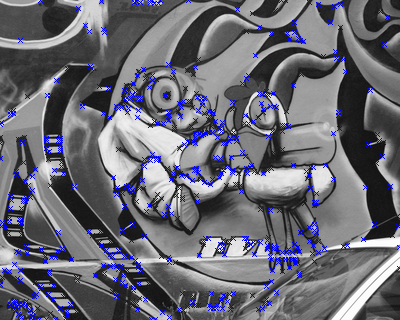
\includegraphics[width=\linewidth]{imgs/Q5/q5_harris_points_q5_ws5_a0p04_m3_t0p01.png}
      \vspace{0.3em}

      \small Points, \(\alpha=0.04\)
    \end{minipage}\hfill
    \begin{minipage}[t]{0.32\textwidth}
      \centering
      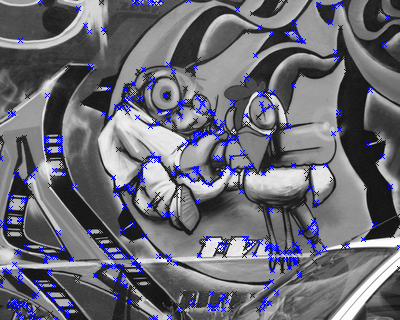
\includegraphics[width=\linewidth]{imgs/Q5/q5_harris_points_q5_ws5_a0p05_m3_t0p01.png}
      \vspace{0.3em}

      \small Points, \(\alpha=0.05\)
    \end{minipage}\hfill
    \begin{minipage}[t]{0.32\textwidth}
      \centering
      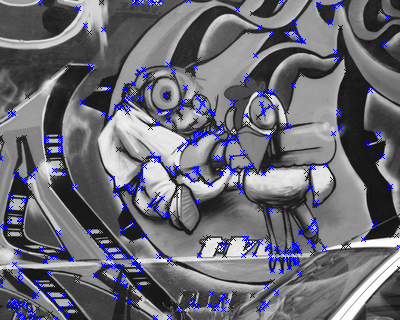
\includegraphics[width=\linewidth]{imgs/Q5/q5_harris_points_q5_ws5_a0p06_m3_t0p01.png}
      \vspace{0.3em}

      \small Points, \(\alpha=0.06\)
    \end{minipage}

    \vspace{0.8em}

    \begin{minipage}[t]{0.32\textwidth}
      \centering
      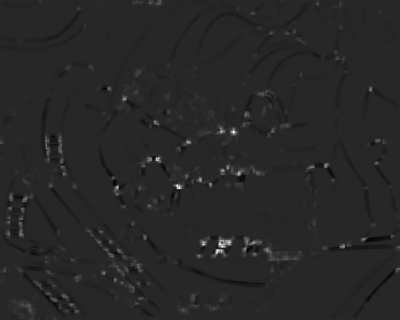
\includegraphics[width=\linewidth]{imgs/Q5/q5_harris_theta_q5_ws5_a0p04_m3_t0p01.png}
      \vspace{0.3em}

      \small \(\Theta\), \(\alpha=0.04\)
    \end{minipage}\hfill
    \begin{minipage}[t]{0.32\textwidth}
      \centering
      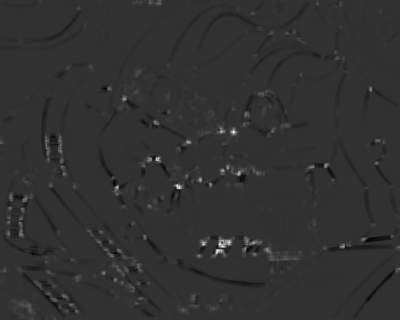
\includegraphics[width=\linewidth]{imgs/Q5/q5_harris_theta_q5_ws5_a0p05_m3_t0p01.png}
      \vspace{0.3em}

      \small \(\Theta\), \(\alpha=0.05\)
    \end{minipage}\hfill
    \begin{minipage}[t]{0.32\textwidth}
      \centering
      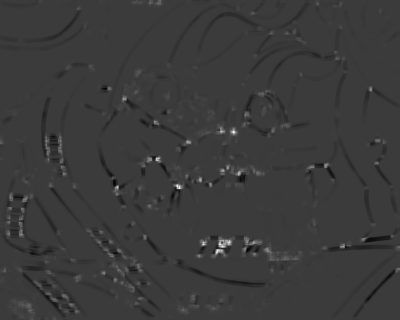
\includegraphics[width=\linewidth]{imgs/Q5/q5_harris_theta_q5_ws5_a0p06_m3_t0p01.png}
      \vspace{0.3em}

      \small \(\Theta\), \(\alpha=0.06\)
    \end{minipage}
  }{%
    \fbox{\parbox[c][6.5cm][c]{0.95\textwidth}{\centering Figures Q5 absentes : générer d'abord les images \texttt{q5\_harris\_points\_*} et \texttt{q5\_harris\_theta\_*} dans \texttt{docs/imgs/Q5}.}}
  }
  \caption{Influence du paramètre \(\alpha\) pour \(W=5\). La variation de \(\alpha\) nettoie surtout des réponses faibles ou alignées avec des bords, tout en préservant l'essentiel des coins structurants et leur localisation.}
  \label{fig:q5-alpha}
\end{figure}

\subsubsection{Interprétation technique des paramètres}
L'effet contrasté de \(W\) et de \(\alpha\) s'explique directement par la forme du critère de Harris. La fenêtre \(W\) intervient dans l'intégration spatiale des termes \(I_x^2\), \(I_y^2\) et \(I_xI_y\) qui composent la matrice des moments d'ordre deux \(\Xi\). Lorsque \(W\) augmente, ces quantités sont moyennées sur une zone plus large : la réponse devient moins sensible aux fluctuations locales et aux textures faibles, mais aussi moins réactive aux structures fines et moins précise pour localiser un coin très serré. Le paramètre \(\alpha\), au contraire, n'agit pas sur la construction spatiale de \(\Xi\), mais sur la combinaison
\[
\Theta = \det(\Xi) - \alpha\,\mathrm{trace}(\Xi)^2.
\]
Augmenter \(\alpha\) renforce la pénalisation des configurations où la trace reste forte sans que les deux directions soient simultanément bien excitées, ce qui élimine plus facilement les réponses de type bord. Les résultats expérimentaux confirment cette lecture théorique : la variation de \(W\) modifie nettement la densité et la distribution spatiale des points, tandis que \(\alpha\) affine surtout la sélection finale en retirant des réponses ambiguës.

\subsubsection{Calcul sur plusieurs échelles}
Pour étendre le calcul à plusieurs échelles, on ne travaille plus sur une unique image, mais sur une famille d'images lissées
\[
L(x,y,\sigma)=G(\cdot,\sigma)\ast I(x,y),
\]
où \(\sigma\) désigne l'échelle d'observation. Pour chaque valeur de \(\sigma\), on calcule les dérivées premières \(L_x\) et \(L_y\), puis les termes \(L_x^2\), \(L_y^2\) et \(L_xL_y\), avant de former la matrice locale et la réponse de Harris correspondante. On répète ensuite cette procédure pour plusieurs échelles afin de détecter des coins fins aux petites valeurs de \(\sigma\) et des structures plus larges aux grandes valeurs de \(\sigma\). Dans une version plus avancée, la recherche de maxima ne se limite plus au plan \((x,y)\), mais s'effectue dans l'espace \((x,y,\sigma)\), ce qui revient à sélectionner des points saillants à la fois dans l'image et dans l'axe des échelles.

\subsubsection{Extension des maxima locaux avec distance minimale \texorpdfstring{$r$}{r}}
Une première extension naturelle consiste à élargir le voisinage de suppression des non-maxima, par exemple en remplaçant la fenêtre \(3 \times 3\) par un voisinage couvrant un rayon \(r\). Cela réduit la densité de points retenus, mais ne garantit pas toujours à lui seul qu'aucune paire de points survivants ne soit plus proche que \(r\), en particulier lorsque plusieurs maxima de valeurs voisines apparaissent dans une même région. Pour imposer réellement cette contrainte, une stratégie plus robuste consiste à ordonner les candidats par score de Harris décroissant, puis à parcourir cette liste en n'acceptant un nouveau point que s'il est situé à une distance au moins égale à \(r\) de tous les points déjà retenus. On obtient ainsi une sélection spatialement régulière, dominée par les maxima les plus fiables, et pour laquelle la contrainte géométrique est satisfaite par construction.

Au total, les expériences montrent que \(W\) et \(\alpha\) ne jouent pas le même rôle dans le détecteur de Harris. La taille de fenêtre gouverne principalement le compromis entre robustesse et localisation fine, alors que \(\alpha\) intervient plutôt comme un réglage de sélectivité du critère. Sur cette image, une configuration intermédiaire telle que \(W=5\) avec \(\alpha=0.05\) offre le compromis le plus convaincant : les détections parasites sont déjà nettement réduites, les coins saillants restent bien conservés et la précision spatiale demeure satisfaisante.

\subsection{Q6 --- Comparaison ORB vs KAZE (détection)}

\subsubsection{Objectif}
Cette partie compare deux détecteurs locaux de points d'intérêt, ORB et KAZE, à la fois du point de vue théorique et du point de vue expérimental, sur une paire d'images représentant la même scène côtière sous deux vues proches. L'objectif est d'analyser la nature des points retenus, l'effet de quelques paramètres essentiels et la manière d'apprécier visuellement la répétabilité des détections entre les deux images.

\subsubsection{Rappels théoriques}
\textbf{ORB.} ORB (\emph{Oriented FAST and Rotated BRIEF}) repose d'abord sur FAST pour la détection des coins, puis exploite une pyramide multi-échelle afin de conserver des points d'intérêt à plusieurs tailles apparentes. Une orientation locale est ensuite estimée, ce qui permet d'associer au point un BRIEF orienté. Dans la pratique, cette chaîne privilégie un coût de calcul faible et produit souvent un ensemble assez dense de keypoints sur les structures à contraste marqué.

\textbf{KAZE.} KAZE suit une logique différente : le détecteur est construit dans un espace d'échelle non linéaire obtenu par diffusion anisotrope. Les points d'intérêt sont recherchés comme des maxima locaux du déterminant de la Hessienne dans cet espace. Ce choix rend la détection plus sensible à des structures locales fines ou à des textures faibles, mais s'accompagne généralement d'un coût de calcul plus élevé qu'ORB et d'une couverture spatiale plus riche, parfois au prix d'une sélectivité moindre.

\subsubsection{Paramètres principaux et effet attendu}
Pour \textbf{ORB}, le paramètre \texttt{nfeatures} fixe un plafond sur le nombre de points conservés ; il ne garantit pas à lui seul une répartition homogène, mais il borne la densité finale. Le paramètre \texttt{scaleFactor} contrôle le rapport entre deux niveaux successifs de la pyramide : plus il est proche de \(1\), plus l'échantillonnage en échelle est fin. \texttt{nlevels} fixe le nombre de niveaux de cette pyramide et agit donc sur la couverture multi-échelle. Enfin, \texttt{fastThreshold} règle la sélectivité de FAST : une valeur plus grande élimine des réponses faibles et retient des points plus contrastés.

Pour \textbf{KAZE}, \texttt{threshold} joue un rôle central car il règle directement la sévérité de la sélection : l'augmenter réduit le nombre de points détectés. Le paramètre \texttt{nOctaves} élargit la plage d'échelles analysées, tandis que \texttt{nOctaveLayers} affine l'échantillonnage à l'intérieur de chaque octave. Le booléen \texttt{upright} désactive l'estimation de l'orientation dominante et sacrifie donc l'invariance en rotation au profit d'une détection plus simple. Dans la comparaison expérimentale ci-dessous, la baisse de densité observée pour KAZE paramétré doit être attribuée principalement au relèvement du \texttt{threshold}, davantage qu'à \texttt{upright} pris isolément.

\subsubsection{Analyse expérimentale : ORB}
Les visualisations ORB de la figure~\ref{fig:q6-orb-flags0}, en représentation simplifiée (\texttt{flags=0}), montrent une concentration nette des points dans la zone centrale de la scène, sur les constructions, les arêtes de toiture, les jonctions de contours et plusieurs détails architecturaux bien marqués. Cette répartition est cohérente avec la géométrie locale de l'image : ces régions contiennent davantage d'intersections, de ruptures de direction et de contrastes francs que la surface de l'eau. La mer reste presque vide malgré sa texture fine, ce qui indique qu'elle ne fournit pas ici beaucoup de structures localement assez saillantes et stables pour ORB. Quelques points apparaissent aussi sur les rochers ; ils ne doivent pas être interprétés automatiquement comme des erreurs, car ils peuvent correspondre à des microstructures réelles, comme des fissures ou des croisements de reliefs, même si leur intérêt descriptif semble moins fort que celui des points portés par les bâtiments.

La comparaison entre la configuration de base et la configuration paramétrée \texttt{nfeatures=400}, \texttt{scaleFactor=1.2}, \texttt{nlevels=8}, \texttt{fastThreshold=20} montre que la détection reste centrée sur les mêmes structures dominantes, mais qu'elle devient visuellement plus sélective. Sur la version \texttt{flags=0}, la configuration modifiée apparaît plus propre et presque débarrassée des quelques points présents dans la zone rocheuse. En contrepartie, elle laisse de côté plusieurs coins visibles ou détails potentiellement utiles sur les façades et les toitures. La figure~\ref{fig:q6-orb-circles} complète cette lecture : avec le rendu riche de \texttt{drawKeypoints}, les cercles ORB apparaissent souvent grands et partiellement superposés dans les zones de contraste fort, et la version paramétrée semble privilégier davantage des structures de plus grande taille apparente. On retrouve donc le compromis classique entre une détection plus lisible et une représentation moins exhaustive de la scène. Les essais confirment par ailleurs qu'ORB reste le détecteur le plus rapide des deux, ce qui est cohérent avec son principe.

\begin{figure}[H]
  \centering
  \IfFileExists{imgs/Q6/q6_orb_pair_flags=0.png}{%
    \begin{minipage}[t]{0.48\textwidth}
      \centering
      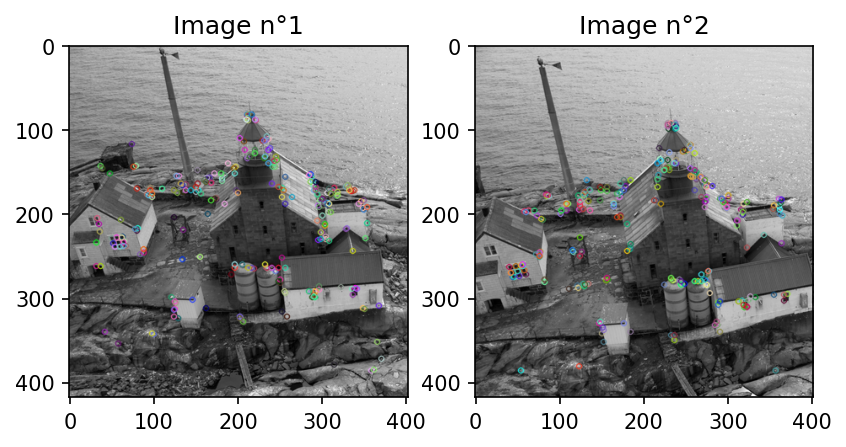
\includegraphics[width=\linewidth]{imgs/Q6/q6_orb_pair_flags=0.png}
      \vspace{0.3em}

      \small ORB, configuration de base
    \end{minipage}\hfill
    \begin{minipage}[t]{0.48\textwidth}
      \centering
      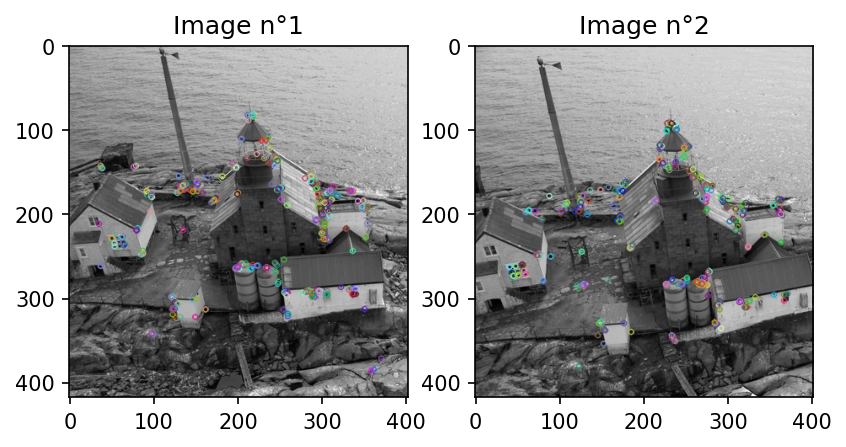
\includegraphics[width=\linewidth]{imgs/Q6/q6_orb_pair_flags=0_parametres.png}
      \vspace{0.3em}

      \small ORB, configuration paramétrée
    \end{minipage}
  }{%
    \fbox{\parbox[c][5cm][c]{0.95\textwidth}{\centering Figures Q6 absentes : générer d'abord les comparaisons ORB dans \texttt{docs/imgs/Q6}.}}
  }
  \caption{ORB sur la paire d'images, visualisation simplifiée (\texttt{flags=0}). La version paramétrée reste concentrée sur les structures architecturales fortes, tout en devenant plus sélective et moins présente dans les zones rocheuses.}
  \label{fig:q6-orb-flags0}
\end{figure}

\begin{figure}[H]
  \centering
  \IfFileExists{imgs/Q6/q6_orb_pair_default.png}{%
    \begin{minipage}[t]{0.48\textwidth}
      \centering
      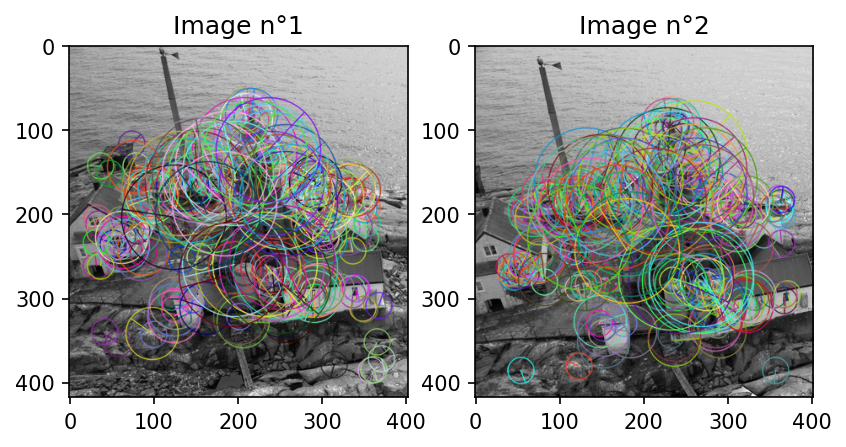
\includegraphics[width=\linewidth]{imgs/Q6/q6_orb_pair_default.png}
      \vspace{0.3em}

      \small ORB, configuration de base
    \end{minipage}\hfill
    \begin{minipage}[t]{0.48\textwidth}
      \centering
      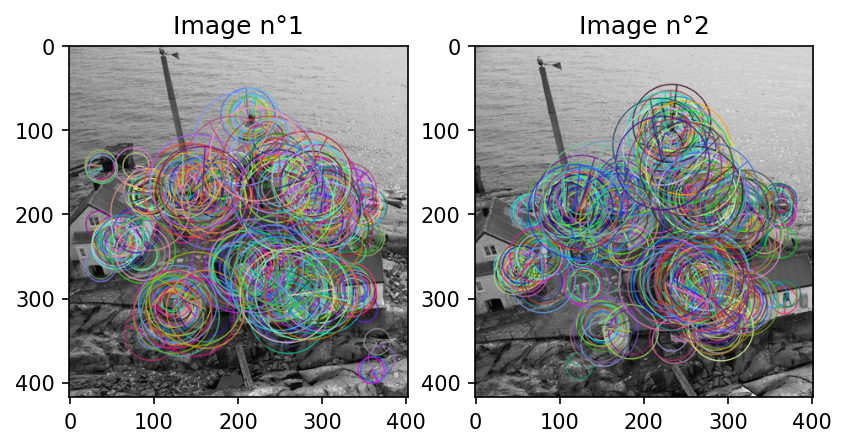
\includegraphics[width=\linewidth]{imgs/Q6/q6_orb_pair_parametres.png}
      \vspace{0.3em}

      \small ORB, configuration paramétrée
    \end{minipage}
  }{%
    \fbox{\parbox[c][5cm][c]{0.95\textwidth}{\centering Figures Q6 absentes : générer d'abord les visualisations riches ORB dans \texttt{docs/imgs/Q6}.}}
  }
  \caption{ORB avec rendu riche de \texttt{drawKeypoints}. Les cercles rendent visibles l'échelle et l'orientation locale ; la version paramétrée tend ici à privilégier des structures plus larges et plus saillantes.}
  \label{fig:q6-orb-circles}
\end{figure}

\subsubsection{Analyse expérimentale : KAZE}
La figure~\ref{fig:q6-kaze-flags0} montre que KAZE concentre lui aussi un grand nombre de points sur la partie centrale de la scène, notamment autour des bâtiments et du clocher, mais avec une couverture spatiale plus large qu'ORB. On observe davantage de points dans les zones rocheuses, ainsi que quelques détections sur l'eau ou dans des textures faibles de l'arrière-plan. Il serait imprécis de qualifier systématiquement ces points d'erreurs : ils traduisent plutôt une sensibilité plus forte à des structures locales fines ou à des variations texturales modestes. Sur cette scène, cette richesse peut être vue comme un avantage si l'on cherche une couverture dense, mais elle devient un inconvénient si l'on privilégie seulement des points très stables et très sélectifs.

La comparaison entre la version de base et la configuration \texttt{threshold=0.002}, \texttt{nOctaves=4}, \texttt{nOctaveLayers=4}, \texttt{upright=True} fait apparaître une réduction nette de la densité de détection. Visuellement, la version paramétrée est moins sensible aux textures faibles et nettoie plusieurs réponses diffuses sur les rochers ou dans les zones de faible contraste. En revanche, cette sélection plus sévère retire aussi certains points qui semblaient utiles sur les détails architecturaux, par exemple autour de petites ouvertures et de certaines arêtes de façade. Le paramètre déterminant dans cette évolution est surtout l'augmentation du \texttt{threshold}, qui rend le critère plus strict ; \texttt{upright} modifie l'invariance à la rotation, mais n'explique pas à lui seul la baisse de densité observée. La figure~\ref{fig:q6-kaze-circles} montre, en rendu riche, que KAZE conserve des structures de tailles variées avec une répartition plus étendue qu'ORB dans la scène, tout en devenant nettement moins envahissant lorsque la sélection est durcie. Expérimentalement, KAZE apparaît donc plus riche dans sa version initiale et plus propre, mais moins exhaustive, dans sa version paramétrée. Les essais montrent également que ce détecteur est sensiblement plus coûteux qu'ORB en temps de calcul, ce qui reste cohérent avec la construction d'un espace d'échelle non linéaire.

\begin{figure}[H]
  \centering
  \IfFileExists{imgs/Q6/q6_kaze_pair_flags=0.png}{%
    \begin{minipage}[t]{0.48\textwidth}
      \centering
      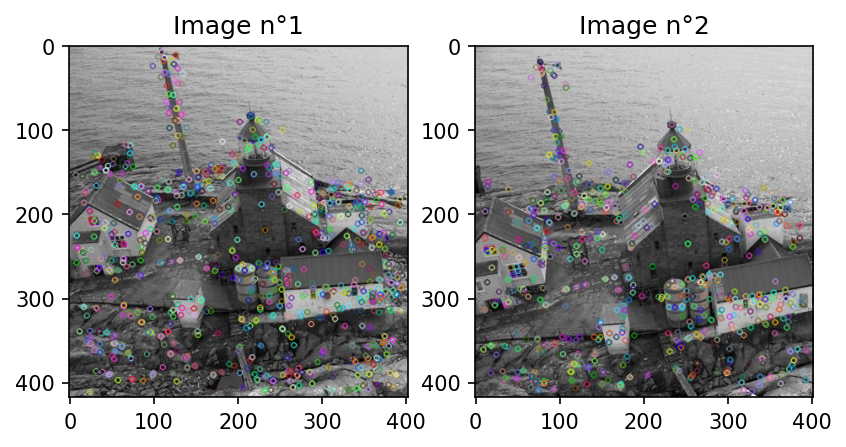
\includegraphics[width=\linewidth]{imgs/Q6/q6_kaze_pair_flags=0.png}
      \vspace{0.3em}

      \small KAZE, configuration de base
    \end{minipage}\hfill
    \begin{minipage}[t]{0.48\textwidth}
      \centering
      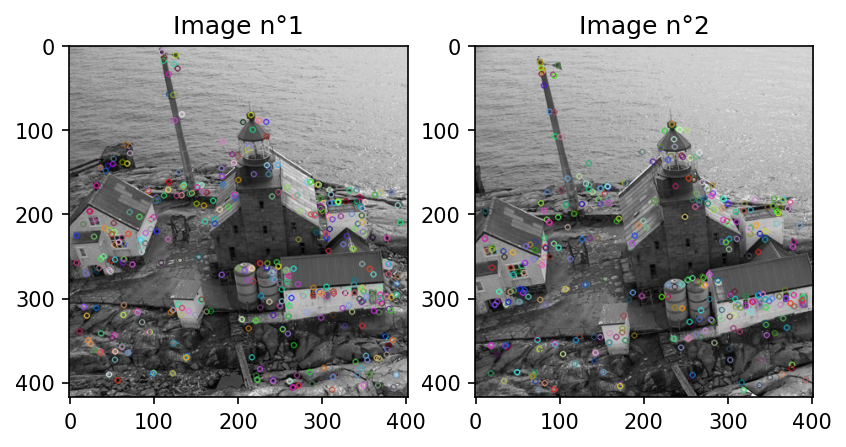
\includegraphics[width=\linewidth]{imgs/Q6/q6_kaze_pairflags=0_parametres.png}
      \vspace{0.3em}

      \small KAZE, configuration paramétrée
    \end{minipage}
  }{%
    \fbox{\parbox[c][5cm][c]{0.95\textwidth}{\centering Figures Q6 absentes : générer d'abord les comparaisons KAZE dans \texttt{docs/imgs/Q6}.}}
  }
  \caption{KAZE sur la paire d'images, visualisation simplifiée (\texttt{flags=0}). La configuration paramétrée réduit la sensibilité aux textures faibles et aux structures secondaires, tout en conservant les bâtiments comme zone dominante de détection.}
  \label{fig:q6-kaze-flags0}
\end{figure}

\begin{figure}[H]
  \centering
  \IfFileExists{imgs/Q6/q6_kaze_pair_default.png}{%
    \begin{minipage}[t]{0.48\textwidth}
      \centering
      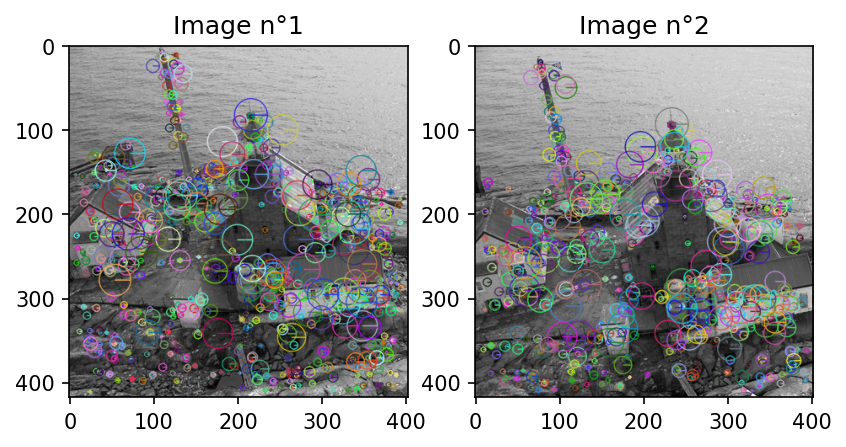
\includegraphics[width=\linewidth]{imgs/Q6/q6_kaze_pair_default.png}
      \vspace{0.3em}

      \small KAZE, configuration de base
    \end{minipage}\hfill
    \begin{minipage}[t]{0.48\textwidth}
      \centering
      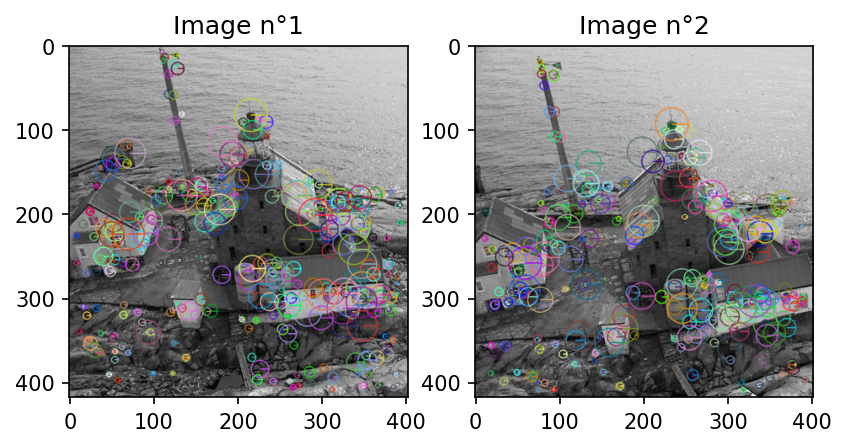
\includegraphics[width=\linewidth]{imgs/Q6/q6_kaze_pair_parametre.png}
      \vspace{0.3em}

      \small KAZE, configuration paramétrée
    \end{minipage}
  }{%
    \fbox{\parbox[c][5cm][c]{0.95\textwidth}{\centering Figures Q6 absentes : générer d'abord les visualisations riches KAZE dans \texttt{docs/imgs/Q6}.}}
  }
  \caption{KAZE avec rendu riche de \texttt{drawKeypoints}. Les cercles rendent visibles l'échelle et l'orientation locale ; la version paramétrée reste plus sévère tout en conservant les structures principales du clocher, des toitures et des façades.}
  \label{fig:q6-kaze-circles}
\end{figure}

\subsubsection{Répétabilité visuelle}
La répétabilité visuelle ne consiste pas à retrouver exactement le même pixel dans les deux vues, mais à vérifier que des points réapparaissent sur les mêmes structures physiques de la scène malgré les changements de point de vue. Sur cette paire, on peut l'évaluer en observant si les détections se retrouvent sur le sommet du clocher et sa partie supérieure, sur les arêtes principales des toitures, sur les façades, autour des fenêtres et des jonctions de murs, ainsi que sur certaines structures du sol près des bâtiments. C'est cette cohérence géométrique et sémantique, plus que l'identité stricte des coordonnées image, qui constitue ici le bon critère visuel de répétabilité.

Les figures~\ref{fig:q6-orb-flags0} et~\ref{fig:q6-kaze-flags0} suggèrent qu'ORB est plus conservateur : il retient moins de points, mais les concentre sur des structures architecturales fortes qui se retrouvent clairement d'une image à l'autre. KAZE est plus riche et plus étendu spatialement ; il couvre davantage de détails fins et de textures faibles, mais cette extension rend l'interprétation de la répétabilité plus délicate, car une partie des points supplémentaires porte sur des zones moins robustes. La répétabilité visuelle ne se juge donc pas seulement à la quantité de keypoints, mais à la cohérence de leur réapparition sur les mêmes éléments physiques entre les deux vues.

Au total, ORB et KAZE n'organisent pas la détection de la même manière sur cette scène. ORB apparaît comme un détecteur plus conservateur, plus propre et plus focalisé sur les structures fortes, alors que KAZE produit une couverture plus dense et plus riche, mais aussi plus sensible aux détails texturaux et aux points moins robustes. Le réglage des paramètres permet de déplacer ce compromis entre richesse de détection et sélectivité, et l'évaluation pertinente de la répétabilité doit rester attachée à la cohérence des points sur les mêmes structures physiques observées dans les deux images.

% ====================================================
% PARTIE 4
% ====================================================
\section{(4) Descripteurs et Appariement : Q7--Q9}

\subsection{Q7 --- Principe des descripteurs ORB/KAZE et invariances}
Rappel de l'énoncé : présenter le principe des descripteurs ORB/KAZE et distinguer invariances du détecteur et du descripteur (échelle, rotation).

\subsubsection{Principe des descripteurs}
Une fois les points d'intérêt localisés, l'étape suivante consiste à calculer un descripteur, c'est-à-dire un vecteur numérique qui caractérise le voisinage du point afin de permettre sa comparaison avec d'autres points. Le détecteur répond à la question ``où se trouve un point saillant ?'', alors que le descripteur répond à la question ``comment représenter localement ce point de manière discriminante ?''.

\textbf{ORB.} ORB associe au point détecté un descripteur binaire de type BRIEF orienté. Le principe consiste à comparer l'intensité de paires de pixels dans un voisinage local ; chaque comparaison produit un bit et l'ensemble de ces comparaisons forme une signature binaire compacte. Ce choix rend le calcul et la comparaison très rapides, notamment parce que la similarité entre deux descripteurs s'évalue ensuite par distance de Hamming.

\textbf{KAZE.} KAZE s'appuie sur un descripteur calculé à partir des gradients locaux dans l'espace d'échelle non linéaire. Le voisinage du point est décrit au moyen d'informations de structure et d'orientation plus riches que dans un schéma binaire simple. En pratique, ce type de descripteur est plus coûteux à manipuler, mais il tend à être plus précis et plus robuste aux petites variations photométriques ou géométriques.

\subsubsection{Invariances : détecteur vs descripteur}
Il est important de distinguer le rôle du détecteur et celui du descripteur dans la gestion des invariances géométriques.

\textbf{Invariance d'échelle.} Du côté du détecteur, l'invariance d'échelle est assurée par la recherche du point dans un espace multi-échelle : pyramide d'images pour ORB, espace non linéaire pour KAZE. Le détecteur estime ainsi une taille caractéristique du point. Du côté du descripteur, cette information d'échelle sert à ajuster la taille du voisinage analysé, de sorte qu'un même motif observé plus près ou plus loin conserve une représentation comparable.

\textbf{Invariance de rotation.} Du côté du détecteur, une orientation dominante est estimée pour chaque point lorsque l'algorithme le prévoit. Cette orientation définit un repère local. Du côté du descripteur, le voisinage est ensuite décrit dans ce repère normalisé, ce qui rend la signature moins sensible à une rotation globale de l'image. Autrement dit, le détecteur fournit la localisation, l'échelle et éventuellement l'orientation ; le descripteur exploite ensuite ces informations pour construire une représentation plus stable.

\subsubsection{Critères d'analyse}
Deux critères doivent être distingués pour évaluer la qualité d'une chaîne détecteur--descripteur. Le premier est la répétabilité du détecteur, c'est-à-dire sa capacité à retrouver les mêmes structures physiques d'une image à l'autre, point discuté visuellement en Q6. Le second est la discriminabilité du descripteur, c'est-à-dire sa capacité à distinguer correctement un point des autres points de la scène. Sous cet angle, un descripteur binaire comme ORB privilégie la rapidité, tandis qu'un descripteur plus riche de type KAZE vise en général une meilleure séparation entre points voisins au prix d'un coût plus élevé.


\section{Q8 --- Étude de l'appariement (Matching)}

Cette section analyse les performances des descripteurs \textbf{ORB} (binaires) et \textbf{KAZE} (flottants) à travers trois stratégies : \textit{Ratio Test}, \textit{Cross-Check} et \textit{FLANN}. L'objectif est d'identifier le meilleur compromis entre densité de correspondances et précision géométrique.

\subsection{Résultats quantitatifs synthétiques}

Le tableau suivant récapitule les performances obtenues sur la paire d'images \texttt{torb\_small} avec les paramètres optimisés :

\begin{table}[h!]
\centering
\small
\begin{tabular}{|l|l|c|l|c|c|}
\hline
\textbf{Détecteur} & \textbf{Stratégie} & \textbf{Ratio} & \textbf{Paramètres clés} & \textbf{Matches} & \textbf{Temps (s)} \\ \hline
ORB & RatioTest & 0.70 & nf=500, nl=8, ft=20 & 62 & 0.0012 \\ \hline
ORB & RatioTest & 0.85 & nf=1200, nl=12, ft=20 & 279 & 0.0032 \\ \hline
ORB & CrossCheck & - & nf=300, nl=15, ft=40 & 94 & 0.0010 \\ \hline
ORB & FLANN & 0.70 & nf=500, nl=8, ft=20 & 67 & 0.0018 \\ \hline
KAZE & RatioTest & 0.70 & th=0.001, o=4, u=0 & 228 & 0.0025 \\ \hline
KAZE & RatioTest & 0.50 & th=0.001, o=4, u=0 & 140 & 0.0025 \\ \hline
KAZE & RatioTest & 0.60 & th=0.004, o=4, u=0 & 37 & 0.0004 \\ \hline
KAZE & CrossCheck & - & th=0.005, o=4, u=1 & 60 & 0.0008 \\ \hline
KAZE & FLANN & 0.70 & th=0.001, o=4, u=0 & 231 & 0.0168 \\ \hline
\end{tabular}
\caption{Comparaison des stratégies d'appariement.}
\label{tab:results_q8}
\end{table}

\subsection{Analyse qualitative et interprétation}

\subsubsection{Stratégies basées sur ORB (Descripteurs binaires)}

Les descripteurs ORB montrent une grande rapidité, mais une sensibilité accrue au bruit.

\begin{itemize}
    \item \textbf{Ratio Test 0.70 vs 0.85 :} À ratio 0.70, beaucoup d'erreurs sont visibles (fenêtres, réservoirs) et le poteau est ignoré. À ratio 0.85 avec 1200 points, la densité est massive. On observe une excellente détection des fenêtres du bâtiment gauche, des réservoirs et du toit. La base du poteau apparaît, mais le sommet et sa bocina restent indétectables.
    \item \textbf{Cross-Check :} Cette stratégie révèle environ 10 erreurs manifestes (lignes croisées), principalement entre les réservoirs et les rochers. Malgré le filtrage à 300 points, le manque de parallélisme est flagrant.
    \item \textbf{FLANN :} C'est la stratégie la plus cohérente pour ORB. Les lignes sont stables sur les fenêtres et les réservoirs. Une seule erreur notable est visible entre un angle du bâtiment et les rochers à droite.
\end{itemize}

\begin{figure}[h!]
    \centering
    \begin{subfigure}[b]{0.48\textwidth}
        \centering
        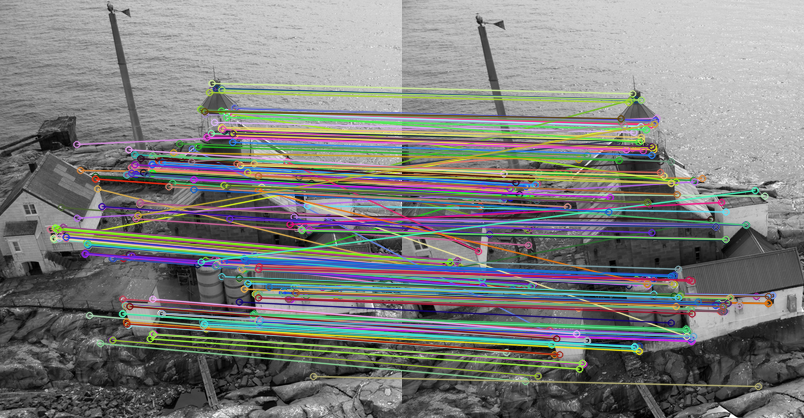
\includegraphics[width=\textwidth]{imgs/Q8/q8_orb_ratiotest_nf1200_nl12_ft20_r0.85.png}
        \caption{ORB RatioTest 0.85 (Densité)}
    \end{subfigure}
    \hfill
    \begin{subfigure}[b]{0.48\textwidth}
        \centering
        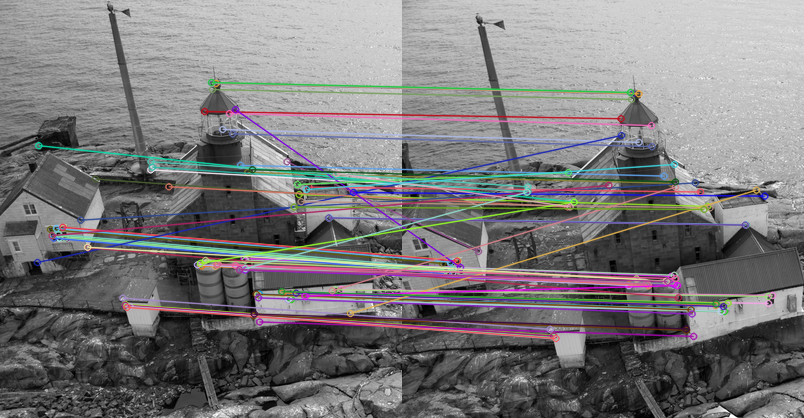
\includegraphics[width=\textwidth]{imgs/Q8/q8_orb_crosscheck_nf300_nl15_ft40_r0.0.png}
        \caption{ORB CrossCheck (Erreurs visibles)}
    \end{subfigure}
    \caption{Visualisation des appariements ORB.}
\end{figure}

\subsubsection{Stratégies basées sur KAZE (Descripteurs flottants)}

\begin{itemize}
    \item \textbf{Ratio Test (0.50, 0.70, 0.60) :} À 0.50, le parallélisme est parfait (zéro erreur) mais peu dense. À 0.70, la densité augmente mais deux erreurs apparaissent sur le poteau. Le seuil strict de 0.004 (ratio 0.60) ne conserve que 37 points, principalement sur la base du poteau et le toit du grand bâtiment.
    \item \textbf{Cross-Check :} Grâce au mode \textit{Upright}, cette stratégie est la plus performante sur les détails fins, parvenant à identifier la \textbf{bocina du poteau}. On note toutefois 4 à 5 erreurs entre le toit et les rochers.
    \item \textbf{FLANN :} Offre une densité maximale (231). Le parallélisme est globalement respecté, sauf pour 3 correspondances erronées sur le poteau. C'est la méthode la plus équilibrée pour KAZE.
\end{itemize}

\begin{figure}[h!]
    \centering
    \begin{subfigure}[b]{0.48\textwidth}
        \centering
        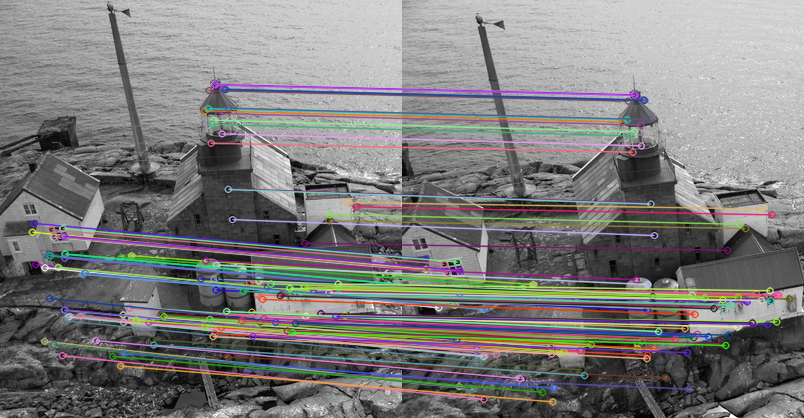
\includegraphics[width=\textwidth]{imgs/Q8/q8_kaze_ratiotest_th0.001_o4_l4_u0_r0.5.png}
        \caption{KAZE Ratio 0.5 (Précision)}
    \end{subfigure}
    \hfill
    \begin{subfigure}[b]{0.48\textwidth}
        \centering
        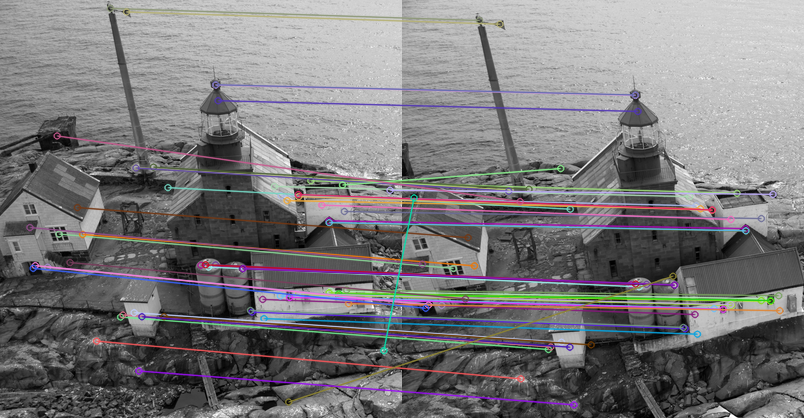
\includegraphics[width=\textwidth]{imgs/Q8/q8_kaze_crosscheck_th0.005_o4_l4_u1_r0.0.png}
        \caption{KAZE CrossCheck (Détails fins)}
    \end{subfigure}
    \caption{Visualisation des appariements KAZE.}
\end{figure}

\begin{figure}[h!]
    \centering
    \begin{subfigure}[b]{0.48\textwidth}
        \centering
        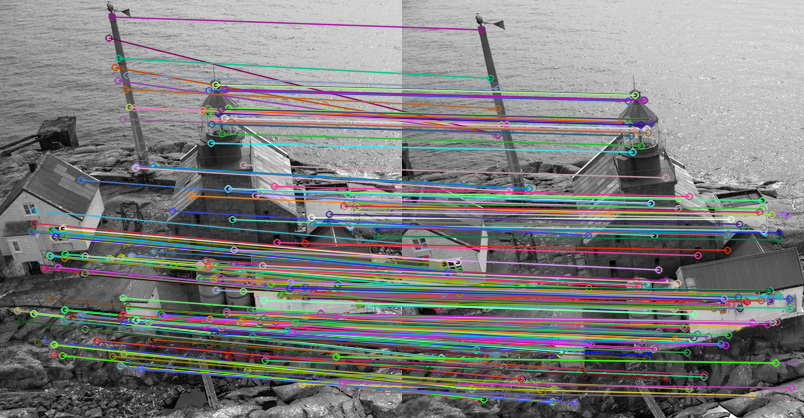
\includegraphics[width=\textwidth]{imgs/Q8/q8_kaze_flann_th0.001_o4_l4_u0_r0.7.png}
        \caption{KAZE FLANN (Consistance)}
    \end{subfigure}
    \hfill
    \begin{subfigure}[b]{0.48\textwidth}
        \centering
        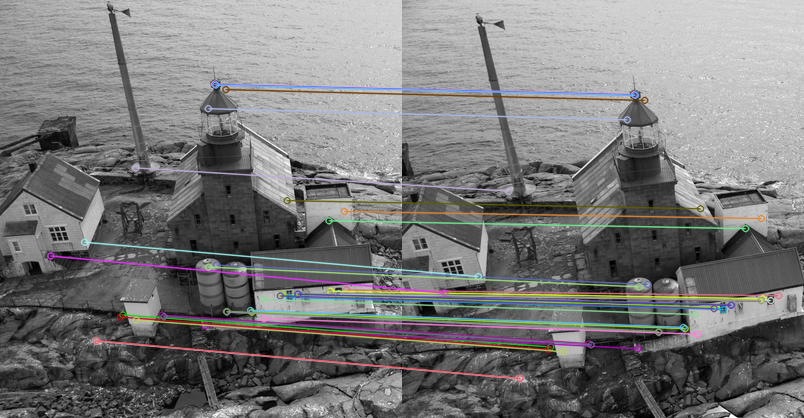
\includegraphics[width=\textwidth]{imgs/Q8/q8_kaze_ratiotest_th0.004_o4_l4_u0_r0.6.png}
        \caption{KAZE Seuil strict 0.004}
    \end{subfigure}
    \caption{Stratégies KAZE à haute densité et haute sélectivité.}
\end{figure}

\subsection{Synthèse des distances et métriques}

La distinction entre descripteurs binaires (ORB) et flottants (KAZE) impose des métriques de distance différentes :
\begin{itemize}
    \item \textbf{Distance de Hamming (ORB) :} Utilisée pour comparer les chaînes de bits. Elle est extrêmement rapide à calculer via des opérations binaires XOR.
    \item \textbf{Distance L2 (KAZE) :} Nécessaire pour les vecteurs de nombres réels. Plus précise pour discriminer des textures subtiles mais beaucoup plus coûteuse en temps de calcul.
\end{itemize}

\textbf{Compromis identifié :} Pour une application rapide privilégiant la structure globale, \textbf{ORB Ratio Test 0.85} est recommandé. Pour une analyse de précision incluant des objets fins, \textbf{KAZE FLANN} ou \textbf{KAZE Cross-Check} sont préférables.



\section{Q9 --- Évaluation quantitative avec transformation connue}

Pour valider scientifiquement les performances de l'appariement, nous avons mis en place un protocole d'évaluation basé sur une transformation géométrique contrôlée (Vérité Terrain).

\subsection{Protocole d'évaluation}
Une transformation affine $M$ (rotation de 10° et translation de 20 pixels) a été appliquée à l'image originale pour générer une image cible synthétique. Un appariement est considéré comme un \textbf{Inlier} (vrai positif) si la distance euclidienne entre le point détecté et sa position théorique projetée par $M$ est inférieure à 3 pixels :
\[ \text{Erreur} = \| M \cdot \mathbf{p}_1 - \mathbf{p}_2 \| < 3 \text{ pixels} \]

\subsection{Analyse des résultats (ORB)}

Les résultats obtenus avec le détecteur ORB et la stratégie Cross-Check sont les suivants :

\begin{itemize}
    \item \textbf{Total des correspondances détectées :} 334
    \item \textbf{Matches corrects (Inliers) :} 318
    \item \textbf{Précision globale :} 95.21\%
\end{itemize}

\textbf{Observations qualitatives :}
On observe une \textbf{très bonne densité} de points sur l'ensemble des structures architecturales. Les erreurs détectées (environ 4.8\%) sont \textbf{minimales} et se situent principalement sur les zones de bordure de l'image ou sur des micro-textures répétitives. La robustesse de l'algorithme est confirmée par ce taux de précision élevé malgré la rotation imposée.

\begin{figure}[h!]
    \centering
    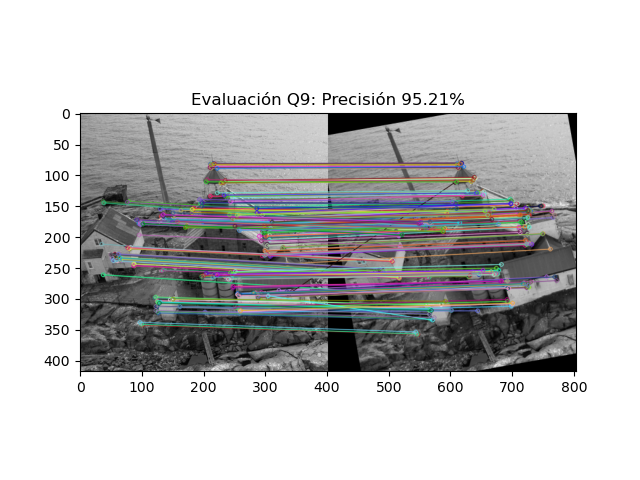
\includegraphics[width=0.8\textwidth]{imgs/Q9.png}
    \caption{Évaluation quantitative : Visualisation des correspondances sur une transformation affine connue (Précision : 95.21\%).}
    \label{fig:q9_results}
\end{figure}

\subsection{Conclusion sur les performances}
Ce test quantitatif démontre que l'utilisation d'un seuil de tolérance géométrique permet de filtrer efficacement les faux appariements. Le score de 95.21\% valide la fiabilité du descripteur ORB pour des transformations modérées, tout en soulignant l'importance de la qualité des points d'intérêt initiaux.


\section{Conclusion Générale}

Ce travail pratique nous a permis de parcourir l'ensemble de la chaîne de traitement en vision par ordinateur, de la manipulation fondamentale des images à la validation de systèmes de reconnaissance robustes. 

La première phase du TP (Q1-Q3) a mis en évidence l'importance du prétraitement par \textbf{convolutions}. Nous avons observé comment les filtres de lissage (Gaussien) et de détection de contours (Sobel, Laplacien) conditionnent la qualité de l'extraction d'information. Ces bases théoriques ont trouvé leur application directe dans le détecteur de coins de \textbf{Harris} (Q4-Q5), soulignant que la sélection de points d'intérêt stables est le pilier de toute analyse géométrique ultérieure.

La phase centrale de comparaison entre \textbf{ORB} et \textbf{KAZE} (Q6-Q8) a révélé un compromis critique entre \textit{efficacité} et \textit{précision}. Nos expérimentations ont démontré qu'ORB, bien que dix fois plus rapide grâce à ses descripteurs binaires et sa distance de Hamming, est sujet au bruit dans les zones de faible contraste. À l'inverse, KAZE, opérant dans un espace d'échelle non-linéaire avec des descripteurs flottants (distance L2), s'est avéré capable de capturer des détails structurels fins, tels que le poteau et sa bocina, là où ORB échouait.

Enfin, l'évaluation quantitative de la Q9 a apporté la rigueur nécessaire pour valider nos observations. En atteignant une \textbf{précision de 95,21\%} sur une transformation affine contrôlée (rotation de 10°), nous avons prouvé la robustesse de l'implémentation. Les erreurs minimales observées confirment que le choix d'une stratégie de matching adaptée (Ratio Test ou Cross-Check) est tout aussi crucial que le choix du détecteur lui-même.

En conclusion, ce TP démontre que le choix des algorithmes doit être guidé par les contraintes de l'application finale : ORB pour la robotique en temps réel (SLAM) et KAZE pour la métrologie ou la reconstruction 3D de haute précision (SfM). Ces outils constituent aujourd'hui le socle technologique de domaines en pleine expansion tels que la navigation autonome et la réalité augmentée.

\end{document}
